% Options for packages loaded elsewhere
\PassOptionsToPackage{unicode}{hyperref}
\PassOptionsToPackage{hyphens}{url}
%
\documentclass[
]{article}
\usepackage{lmodern}
\usepackage{amssymb,amsmath}
\usepackage{ifxetex,ifluatex}
\ifnum 0\ifxetex 1\fi\ifluatex 1\fi=0 % if pdftex
  \usepackage[T1]{fontenc}
  \usepackage[utf8]{inputenc}
  \usepackage{textcomp} % provide euro and other symbols
\else % if luatex or xetex
  \usepackage{unicode-math}
  \defaultfontfeatures{Scale=MatchLowercase}
  \defaultfontfeatures[\rmfamily]{Ligatures=TeX,Scale=1}
\fi
% Use upquote if available, for straight quotes in verbatim environments
\IfFileExists{upquote.sty}{\usepackage{upquote}}{}
\IfFileExists{microtype.sty}{% use microtype if available
  \usepackage[]{microtype}
  \UseMicrotypeSet[protrusion]{basicmath} % disable protrusion for tt fonts
}{}
\makeatletter
\@ifundefined{KOMAClassName}{% if non-KOMA class
  \IfFileExists{parskip.sty}{%
    \usepackage{parskip}
  }{% else
    \setlength{\parindent}{0pt}
    \setlength{\parskip}{6pt plus 2pt minus 1pt}}
}{% if KOMA class
  \KOMAoptions{parskip=half}}
\makeatother
\usepackage{xcolor}
\IfFileExists{xurl.sty}{\usepackage{xurl}}{} % add URL line breaks if available
\IfFileExists{bookmark.sty}{\usepackage{bookmark}}{\usepackage{hyperref}}
\hypersetup{
  pdfauthor={Sumadhuri Damerla,Shaoor Jan,Ashjan Khan},
  hidelinks,
  pdfcreator={LaTeX via pandoc}}
\urlstyle{same} % disable monospaced font for URLs
\usepackage[margin=1in]{geometry}
\usepackage{graphicx,grffile}
\makeatletter
\def\maxwidth{\ifdim\Gin@nat@width>\linewidth\linewidth\else\Gin@nat@width\fi}
\def\maxheight{\ifdim\Gin@nat@height>\textheight\textheight\else\Gin@nat@height\fi}
\makeatother
% Scale images if necessary, so that they will not overflow the page
% margins by default, and it is still possible to overwrite the defaults
% using explicit options in \includegraphics[width, height, ...]{}
\setkeys{Gin}{width=\maxwidth,height=\maxheight,keepaspectratio}
% Set default figure placement to htbp
\makeatletter
\def\fps@figure{htbp}
\makeatother
\setlength{\emergencystretch}{3em} % prevent overfull lines
\providecommand{\tightlist}{%
  \setlength{\itemsep}{0pt}\setlength{\parskip}{0pt}}
\setcounter{secnumdepth}{5}

\usepackage{etoolbox}
\makeatletter
\providecommand{\subtitle}[1]{% add subtitle to \maketitle
  \apptocmd{\@title}{\par {\large #1 \par}}{}{}
}
\makeatother
\subtitle{Final Report}
\author{Sumadhuri Damerla,Shaoor Jan,Ashjan Khan}
\date{}

\begin{document}

{
\setcounter{tocdepth}{2}
\tableofcontents
}
\hypertarget{introduction-to-the-dataset}{%
\section{Introduction to the
dataset}\label{introduction-to-the-dataset}}

\hypertarget{data-source}{%
\subsection{Data source}\label{data-source}}

The data source used for this analysis is the \emph{2018 google play
store}(\url{https://www.kaggle.com/lava18/google-play-store-apps})
collected from Kaggle.

\hypertarget{description-of-the-dataset}{%
\subsection{Description of the
dataset}\label{description-of-the-dataset}}

The dataset is a collection of web-scraped data of 10,000 apps from
Google Play Store. Google Play Store originally referred as the Android
Market, is Google's official store and portal for Android apps, games
and other content for Android-powered phone, tablet or Android TV
device. As of May 2017, it has over two billion monthly active users,
the largest installed base of any operating system, and as of January
2020, the Google Play Store features over 2.9 million apps{[}13{]}.

The variables of the dataset are as follows:

\begin{enumerate}
\def\labelenumi{\arabic{enumi})}
\tightlist
\item
  App (Name) -- Name/Title of the application
\item
  Category (App)- Category/Domain to which the app belongs to
\item
  Rating (App)- Overall user rating of the app
\item
  Reviews (User)- Number of user reviews for the app
\item
  Size (App)- Space or memory that the app takes up
\item
  Installs (App)- Number of user downloads/installs
\item
  Type (Free/Paid)-Apps may be free or paid depending on the developer's
  choice
\item
  Price (App)-Price of the app if not free
\item
  Content Rating - Age group the app is based off at - Children / Mature
  21+ / Adult
\item
  Genres (Detailed Category)- An app can belong to multiple genres, For
  eg, a musical family game will belong to Music, Game, Family genres.
\item
  Last Updated (App)- Date when the app was last updated on Play Store
\item
  Current Version (App)- Current version of the app available on Play
  Store\\
\item
  Android Version (Support) -- minimum version of android it takes to
  have the app on the device
\end{enumerate}

\hypertarget{purpose-of-the-project}{%
\section{Purpose of the project}\label{purpose-of-the-project}}

\begin{itemize}
\item
  The aim of our project is to find out if we can predict ratings of an
  app based on different variables and we intend to summarise the
  different factors that influence the success of an app.These analysis
  might also help the developer community to build more successful apps
  by taking accurate data-based decisions, and focusing on those aspects
  of applications that matters most.
\item
  Also,since this is the first time we are doing data analysis using R,
  it is a fun way to learn and to strengthen the concepts learned during
  the course by taking a hands-on approach.
\end{itemize}

\hypertarget{intended-audience-of-the-project}{%
\section{Intended audience of the
project}\label{intended-audience-of-the-project}}

\begin{itemize}
\item
  We believe there's a diverse set of audience who might be interested
  in our project. As of Febraury 2020, 73.3\% of the mobile operating
  system market share belongs to Android devices{[}11{]}. This large
  community consists of the general public who use android devices and
  appstore,the developer community and anyone who wants to understand
  how the app market works.
\item
  This project is primarily intended for the growing developer
  community. It will help them make data backed decisions before
  launching their application. Besides developers, it is also helpful
  for tech journalists, Google Play Store users or any other interested
  party.
\end{itemize}

\hypertarget{exploratory-data-analysis-to-find-factors-for-success-of-an-app}{%
\section{Exploratory Data Analysis to find factors for success of an
app}\label{exploratory-data-analysis-to-find-factors-for-success-of-an-app}}

Generally, the most successful apps have high ratings and high
installs.To look at which app makes it to the top, we consider ratings
and installs, so we explore these to find any relationship or trends

\hypertarget{rating-column-in-depth}{%
\subsection{Rating column in depth}\label{rating-column-in-depth}}

\hypertarget{distribution-of-rating}{%
\subsubsection{Distribution of rating}\label{distribution-of-rating}}

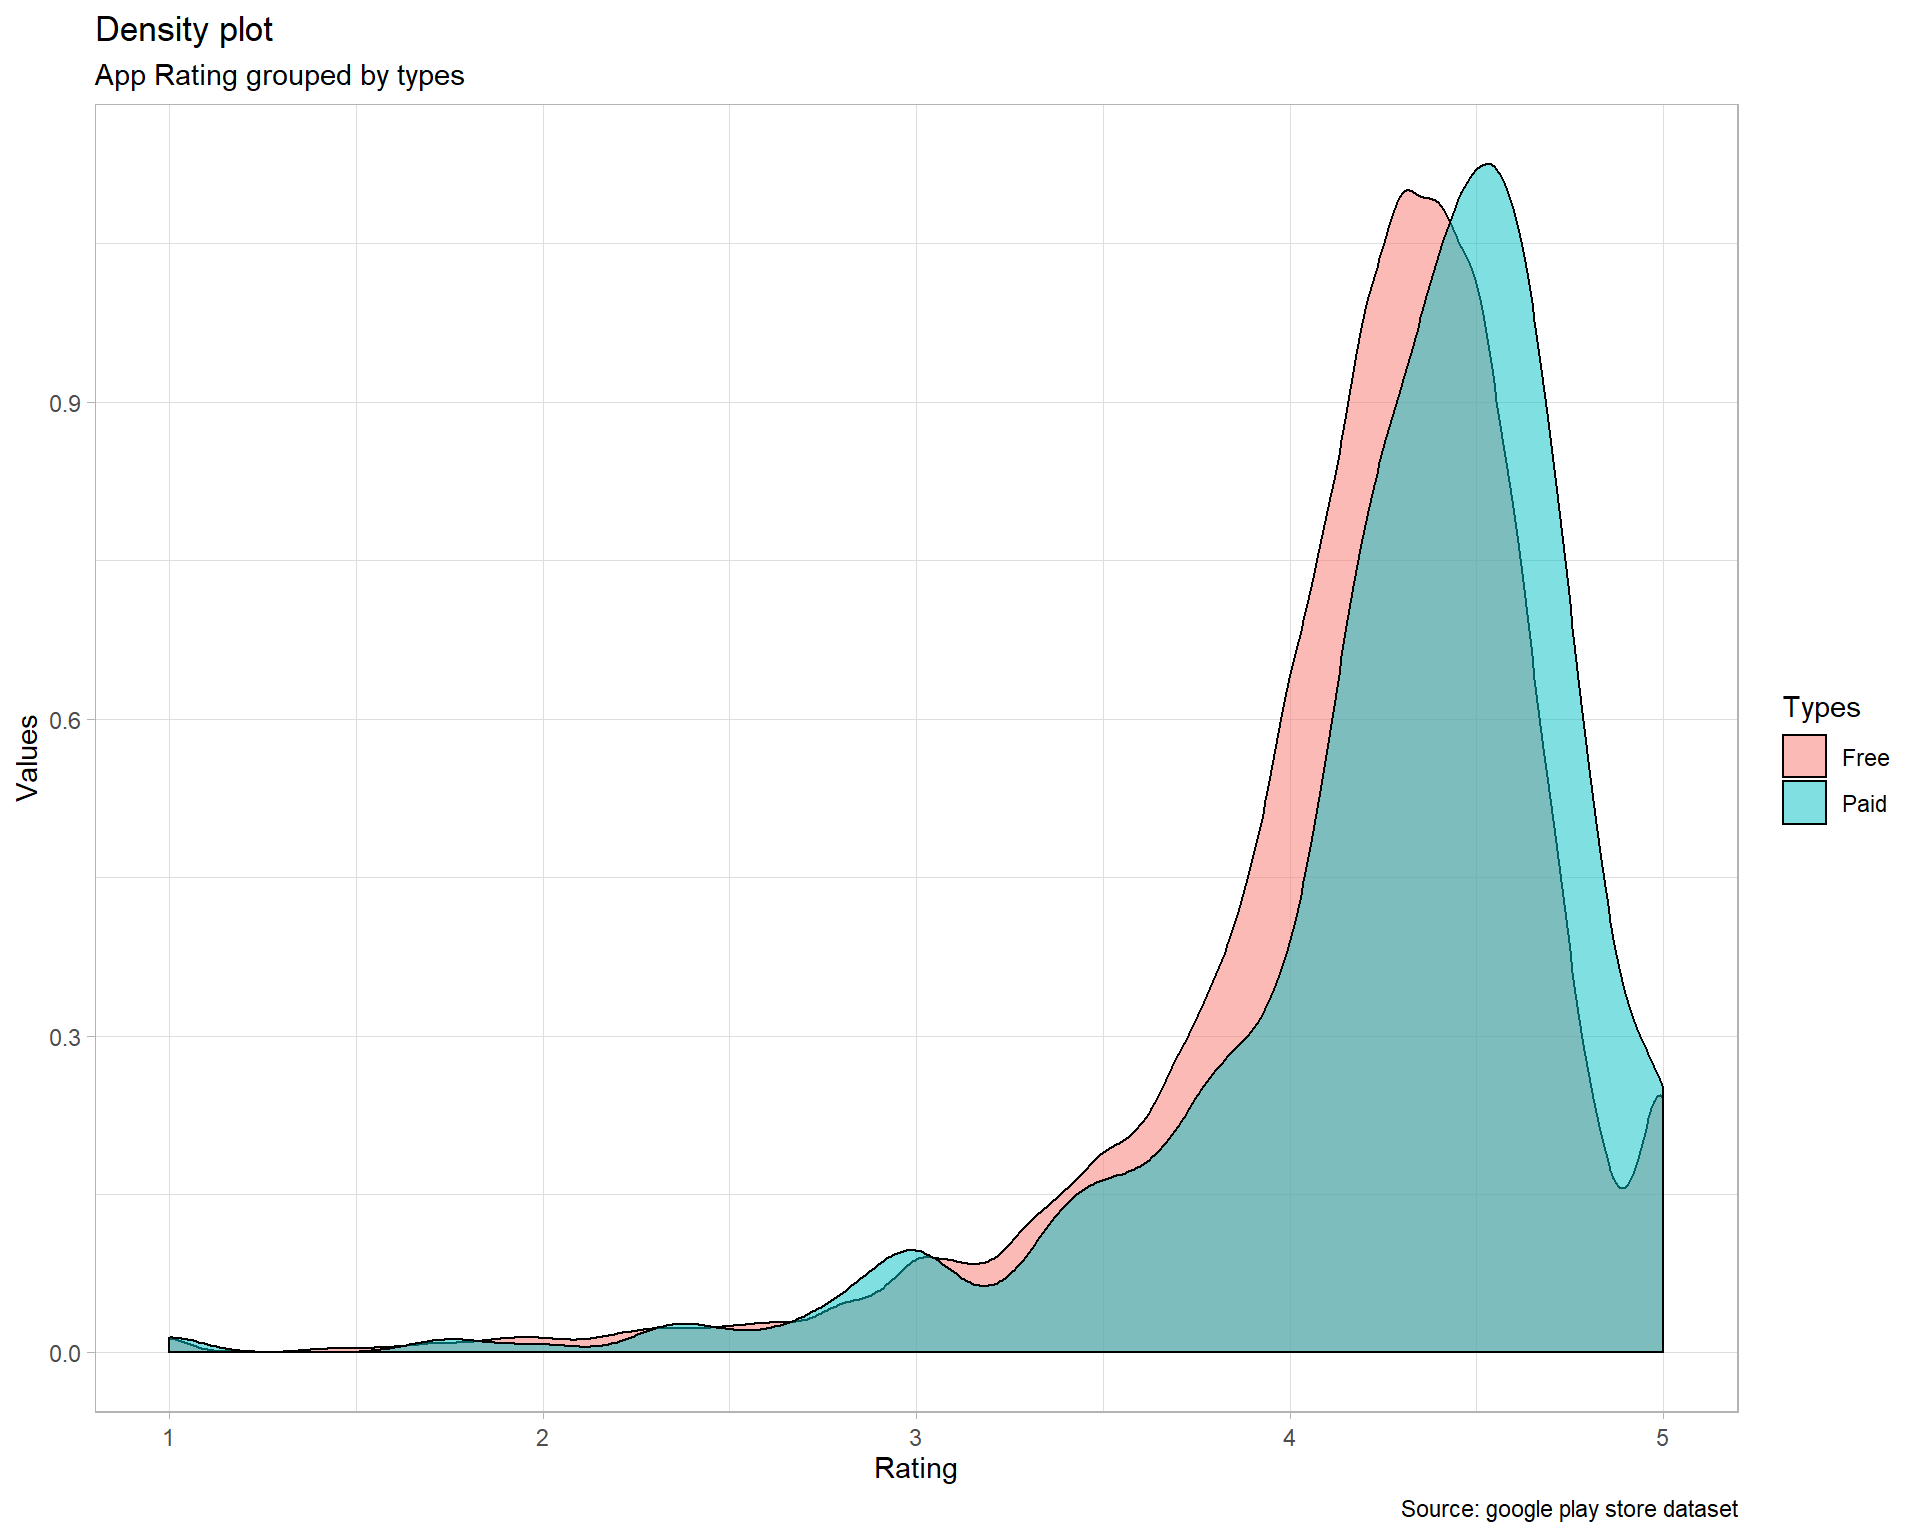
\includegraphics{Group3_final_report_files/figure-latex/rating-density-plot-1.pdf}

\begin{itemize}
\tightlist
\item
  We can observe that the number of apps with low ratings are less in
  number, and most apps have a ratings between 3-5.
\end{itemize}

First, we plot correlograms of ratings versus different columns to find
any relationship. Correlograms are useful to understand the relationship
between different numerical variables. If the correlogram index is 1, it
means that the variables are directly proportional to each other.

\hypertarget{correlogram-plots}{%
\subsection{Correlogram plots}\label{correlogram-plots}}

\begin{center}\includegraphics[width=0.5\linewidth]{Group3_final_report_files/figure-latex/correlogram-plot-1} \includegraphics[width=0.5\linewidth]{Group3_final_report_files/figure-latex/correlogram-plot-2} \includegraphics[width=0.5\linewidth]{Group3_final_report_files/figure-latex/correlogram-plot-3} \includegraphics[width=0.5\linewidth]{Group3_final_report_files/figure-latex/correlogram-plot-4} \end{center}

\includegraphics[width=0.5\linewidth]{Group3_final_report_files/figure-latex/correlogram_type-1}

\textbf{Finding:}\\
+ Each correlation index talks about the relationship between plotted
columns. If the index is 1, it means they have linear relationship +
Each plot on the diagonal refers to the density plot of the respective
column\\
+ We can observe that there is no significant linear relationship
between rating and the plotted numerical variables.

\hypertarget{plot-of-reviews-vs-app-ratings}{%
\subsubsection{Plot of reviews vs app
ratings}\label{plot-of-reviews-vs-app-ratings}}

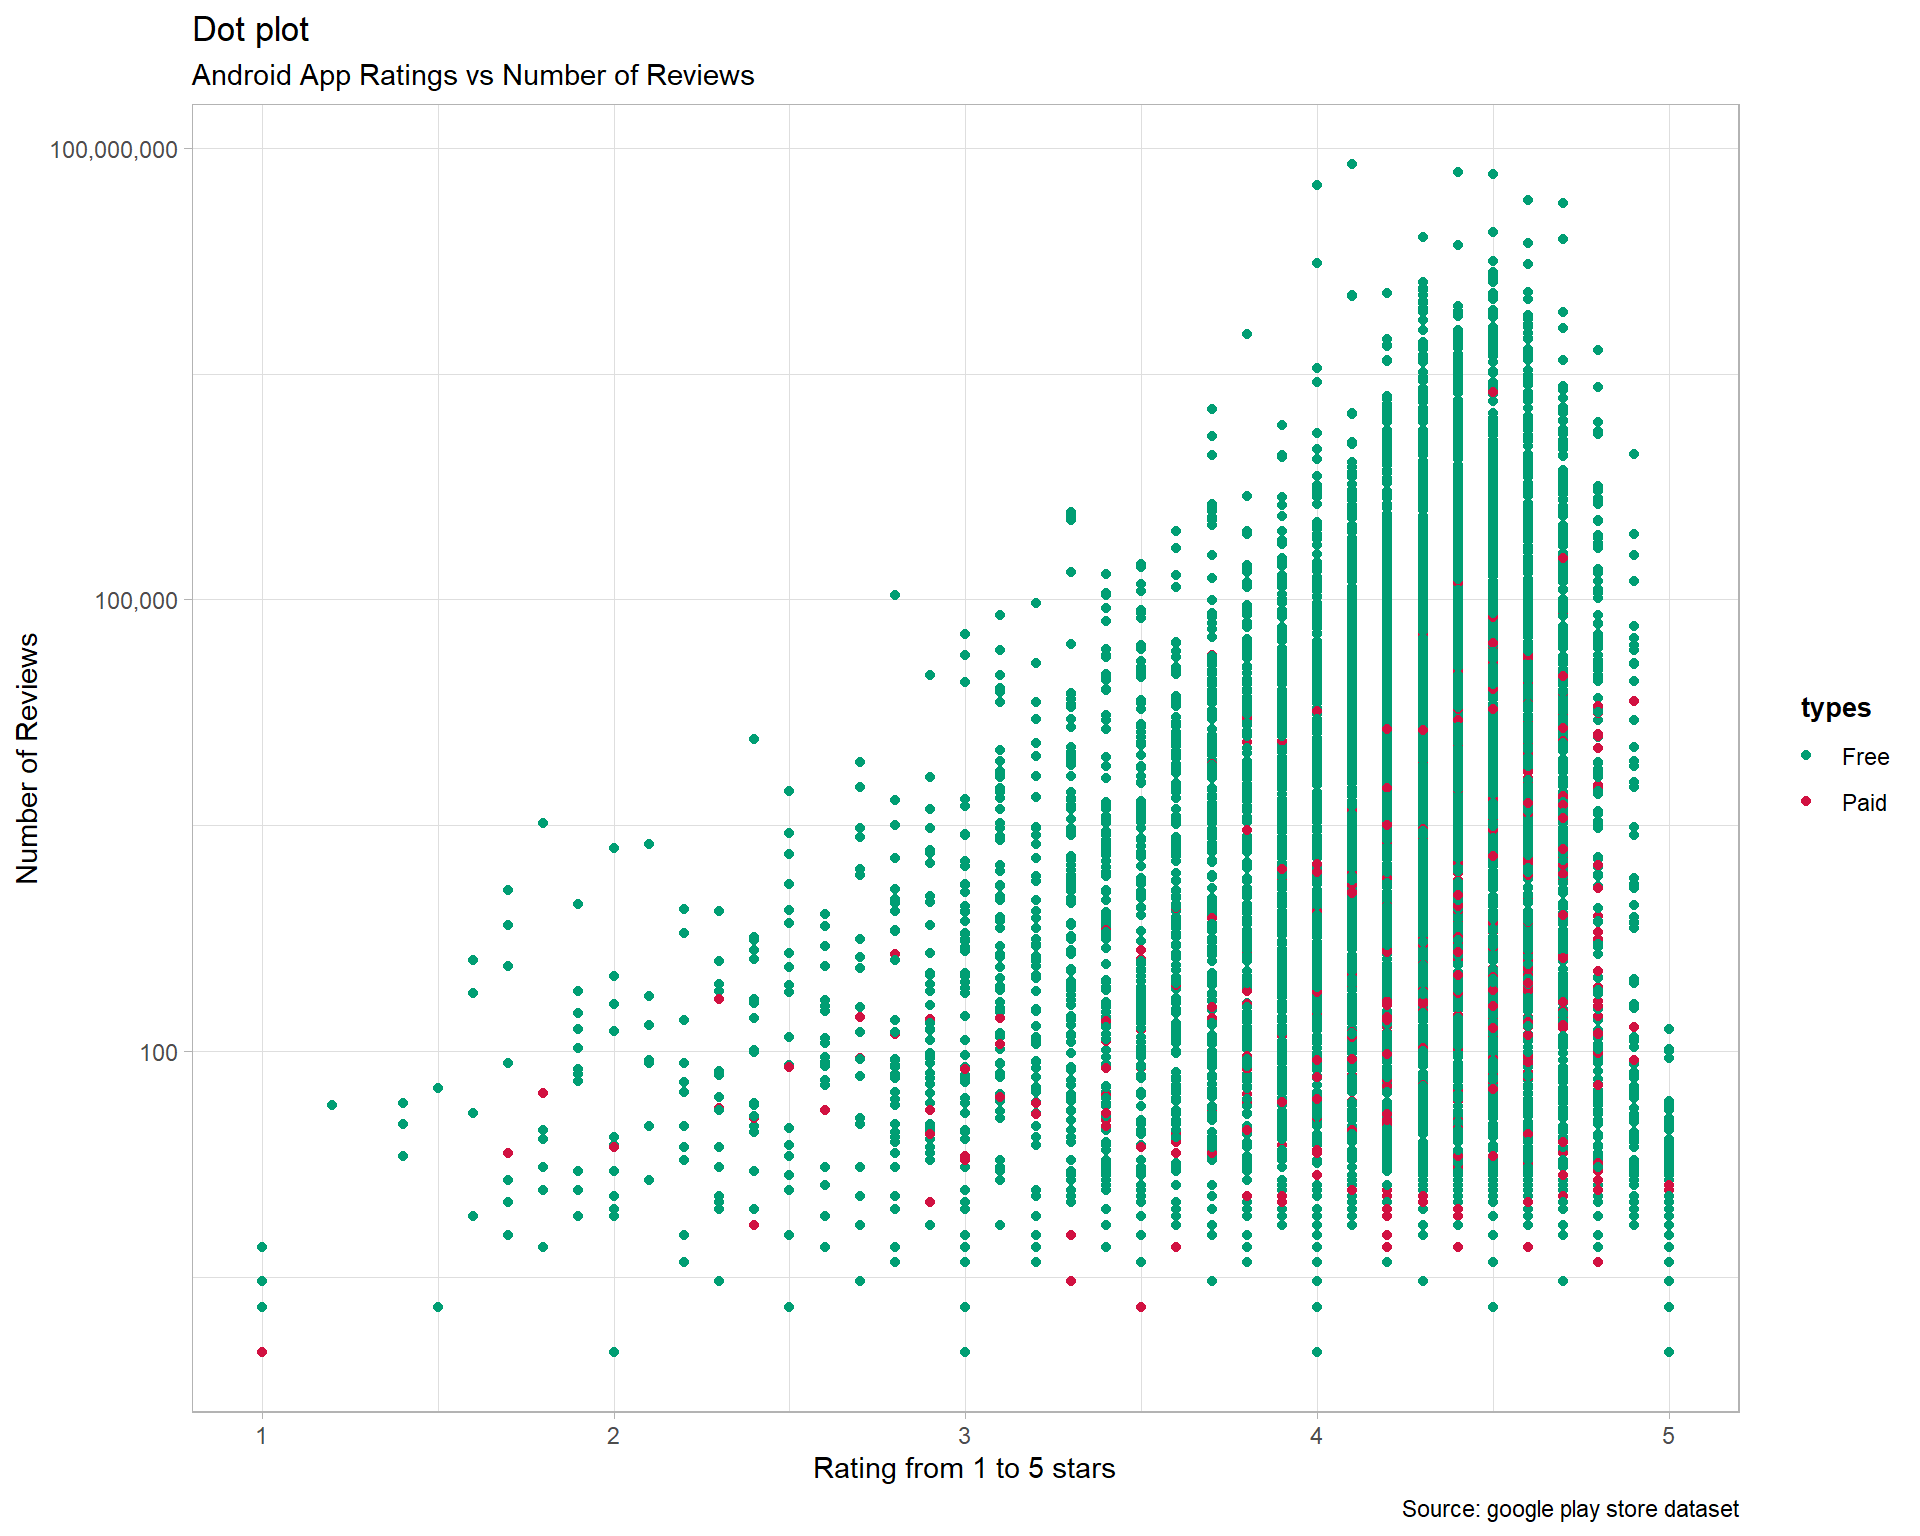
\includegraphics{Group3_final_report_files/figure-latex/review-rating-plot-1.pdf}

\textbf{Finding:} We can observe that the number of reviews influence
the ratings. Generally, as the number of reviews increase, the rating is
higher.

We now explore other factors that might potentially influence rating

\hypertarget{app-rating-vs-category}{%
\subsubsection{App rating vs category}\label{app-rating-vs-category}}

To check the relationship between category and rating, we plotted a box
plot with rating on y-axis and category on x-axis.\\
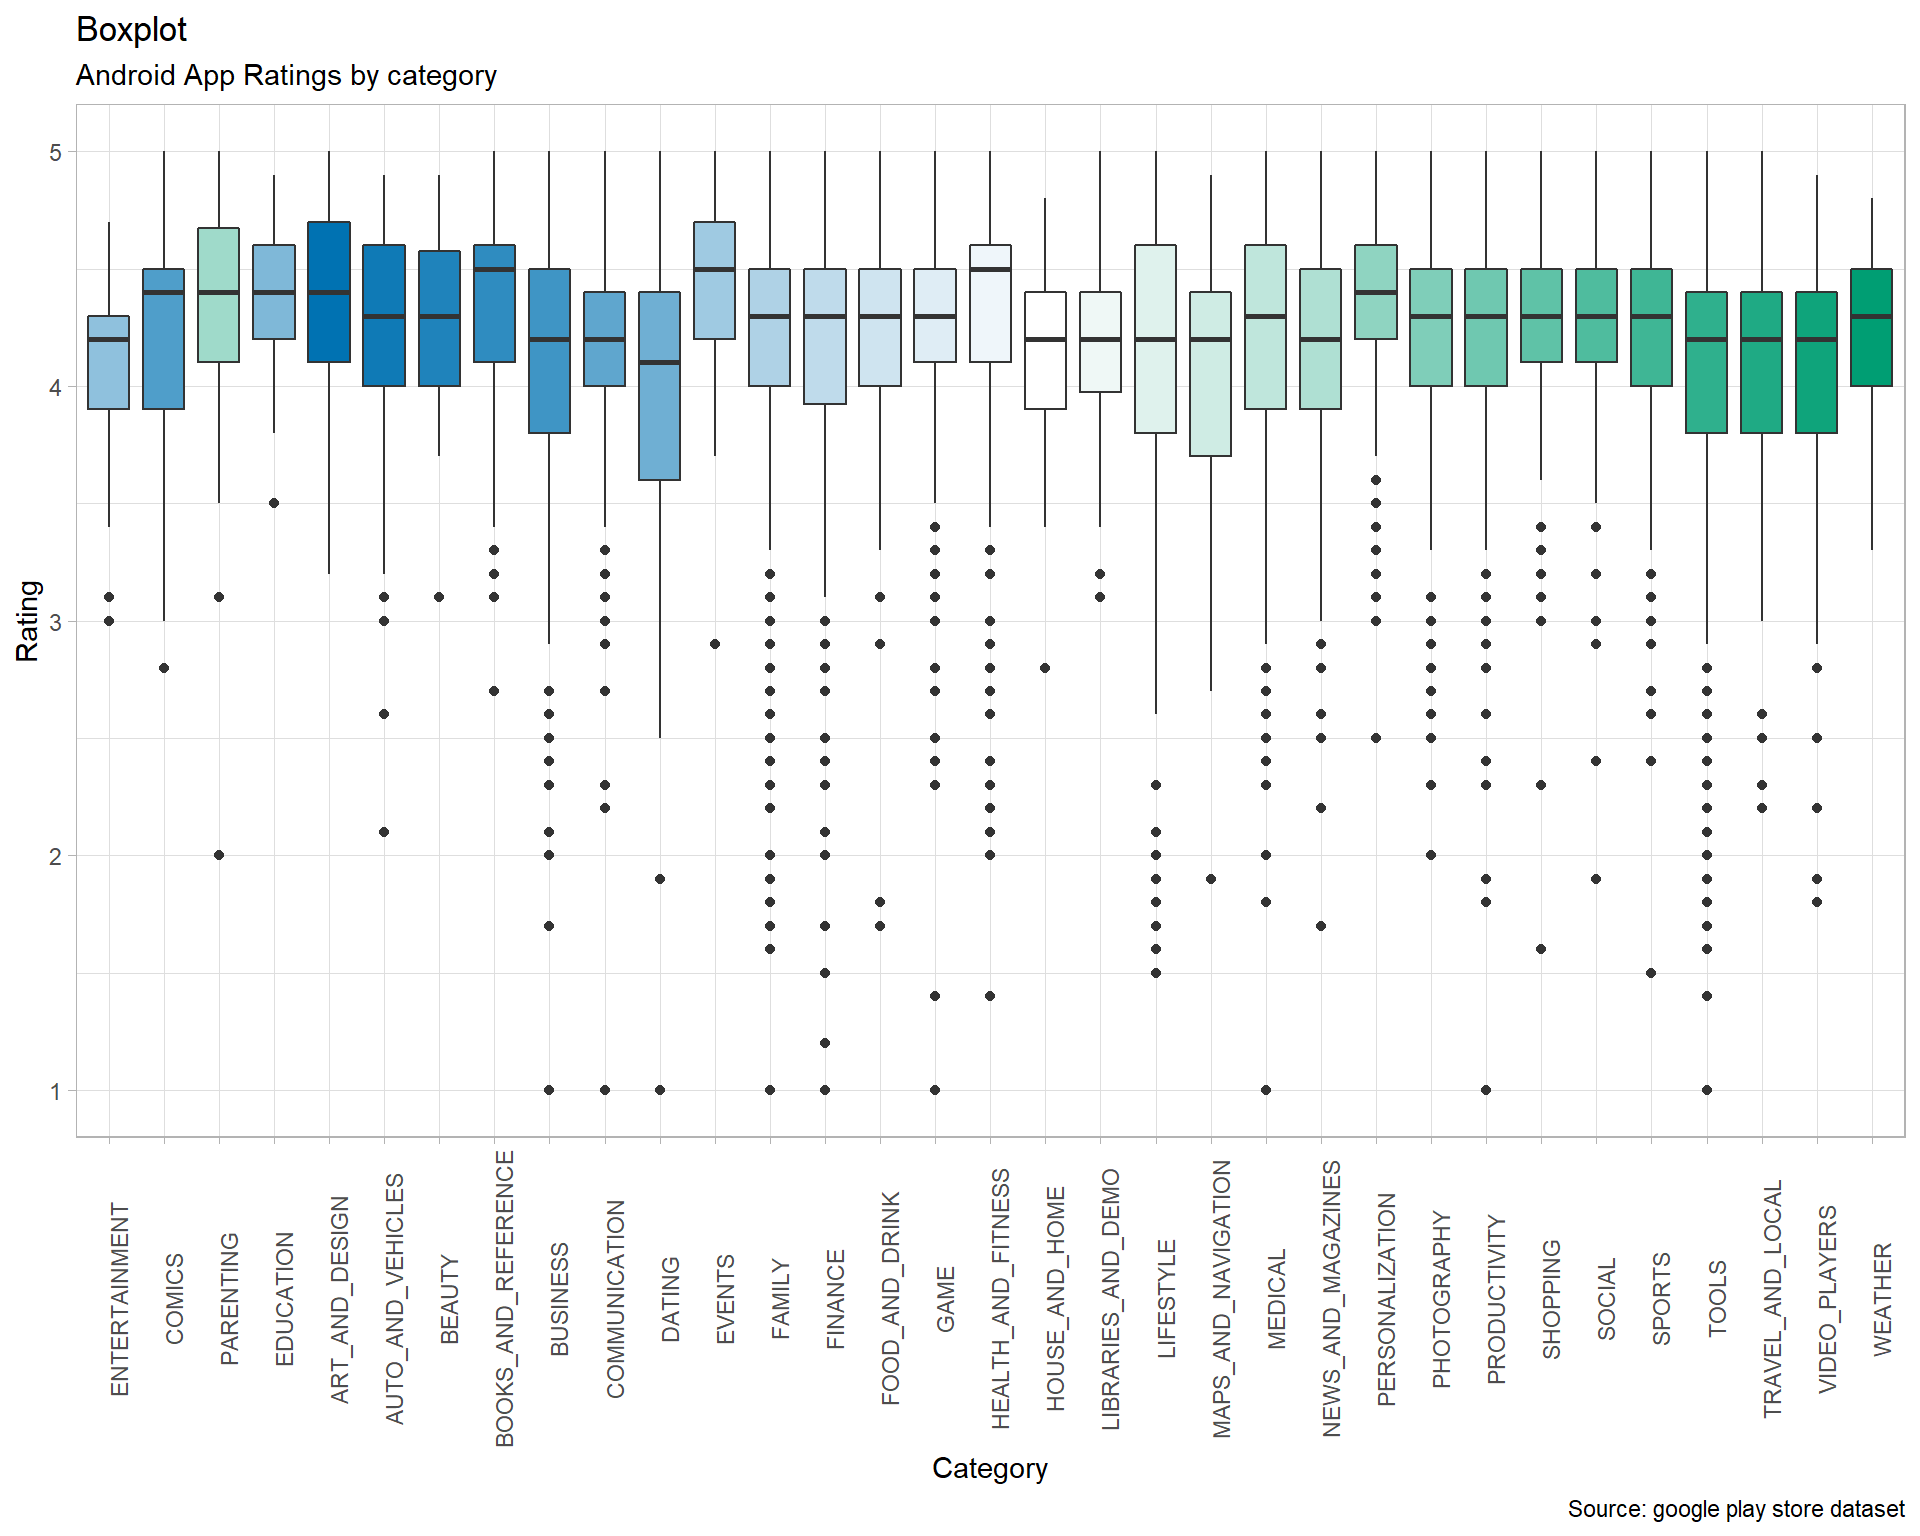
\includegraphics{Group3_final_report_files/figure-latex/rating-category-plot-1.pdf}

\textbf{Finding:} This graph shows that for some categories like TOOLS,
FAMILY, FINANCE and LIFESTYLE a great majority of applications fall
below first quartile. Thus, even though median rating is high, deviation
from median is significant.

\hypertarget{distribution-of-rating-for-8-categories-with-the-largest-numbers-of-apps}{%
\subsubsection{Distribution of rating for 8 categories with the largest
numbers of
apps}\label{distribution-of-rating-for-8-categories-with-the-largest-numbers-of-apps}}

Here we look at the distribution of rating across different categories.
We chose 8 categories with the largest number of applications.

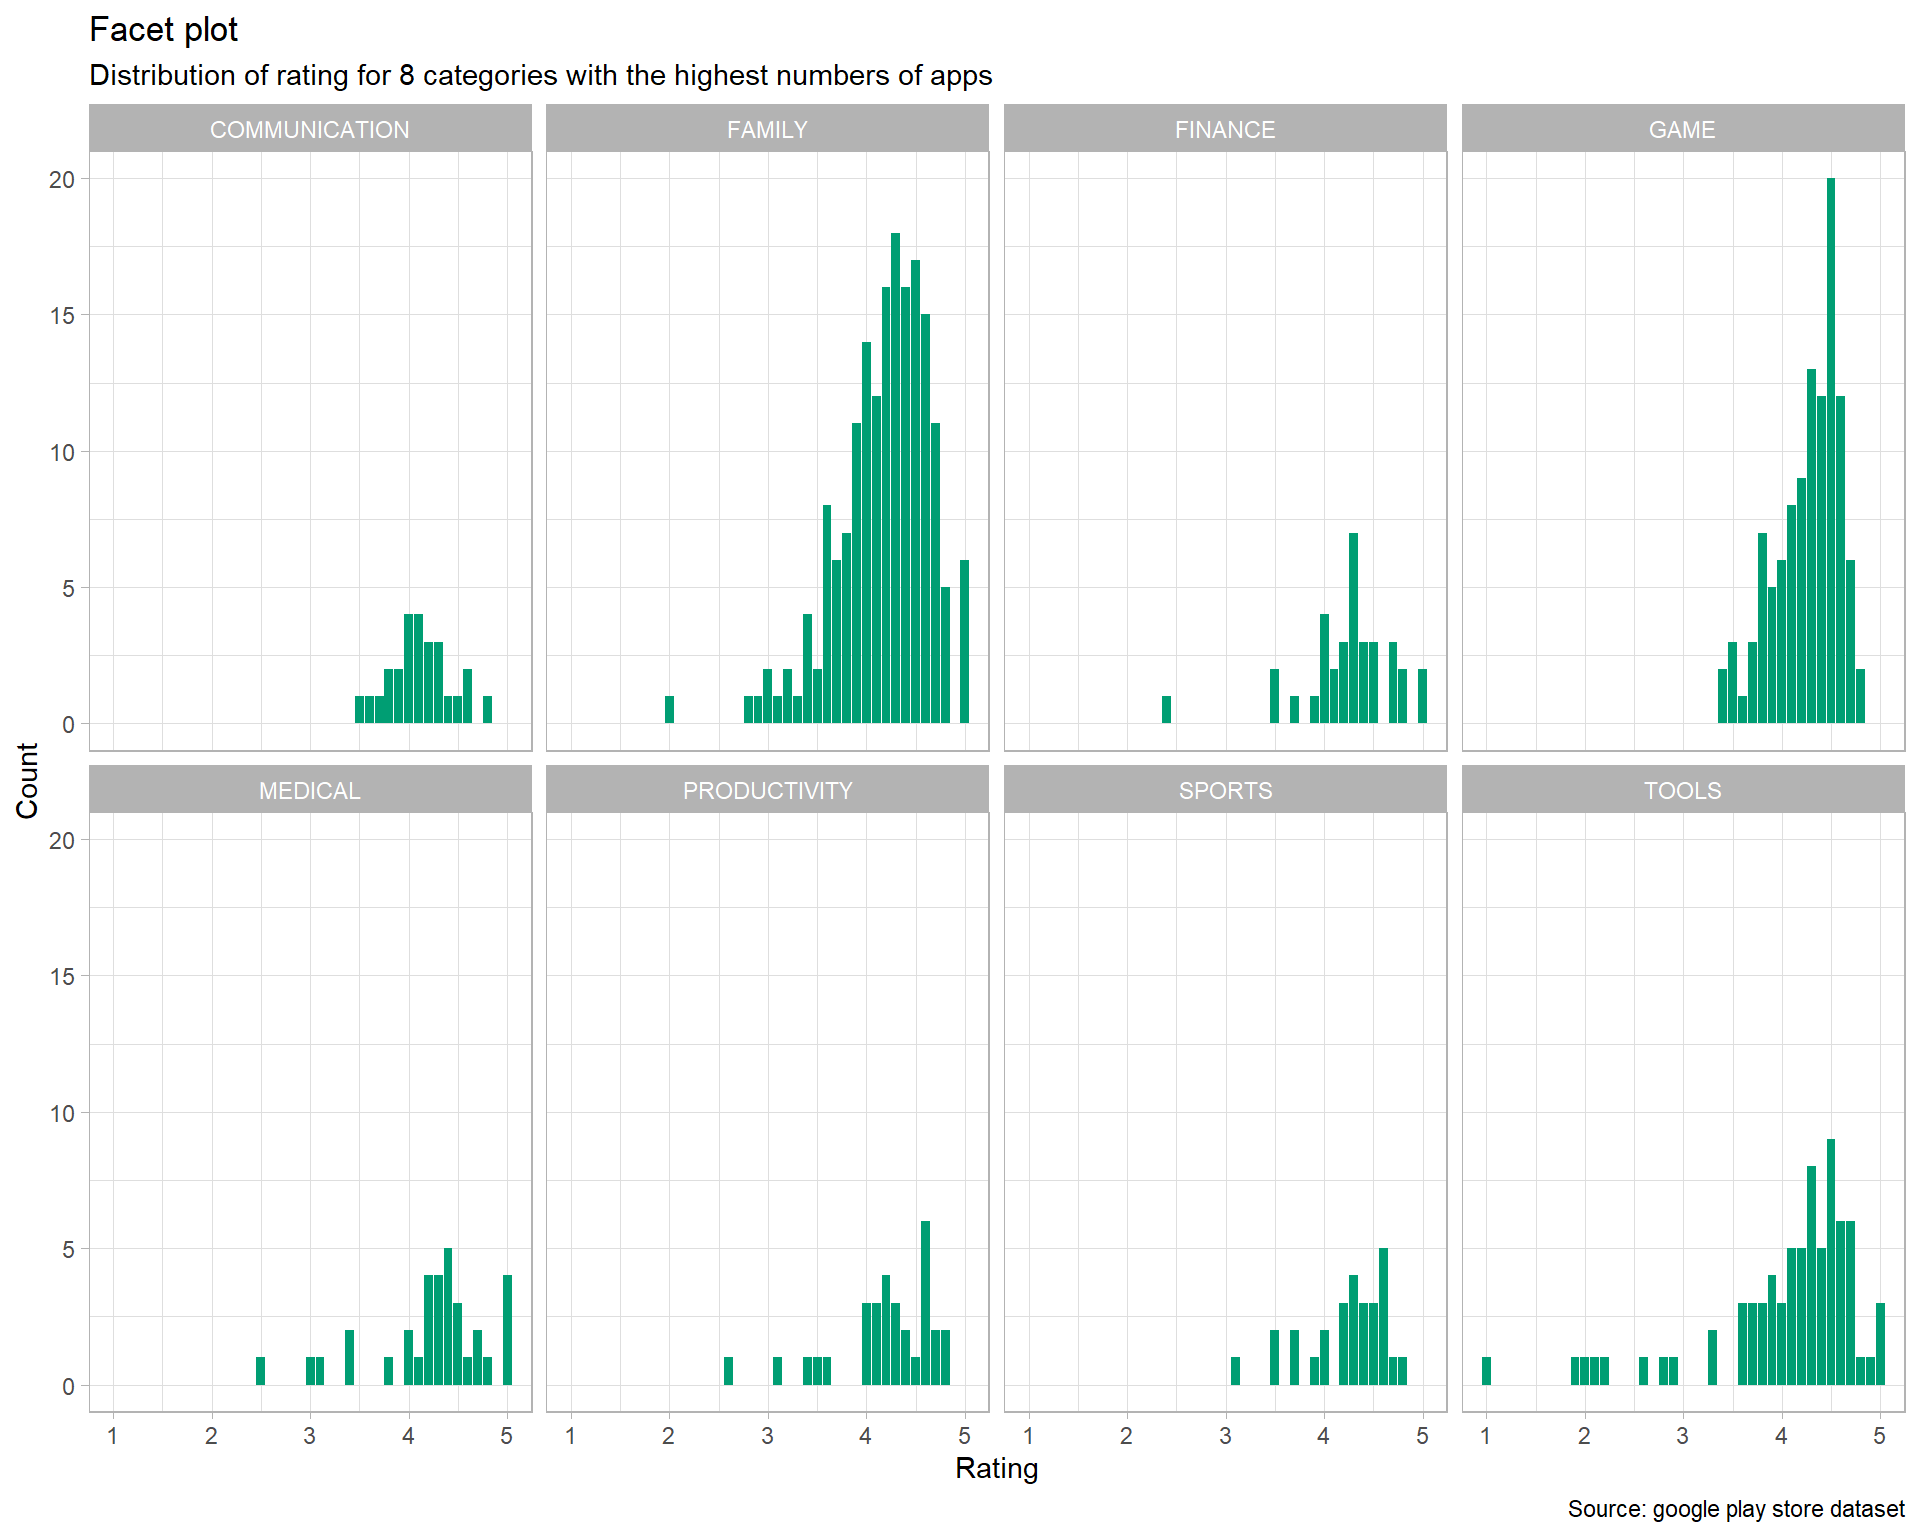
\includegraphics{Group3_final_report_files/figure-latex/avg-rating-distributionplot-1.pdf}

\textbf{Finding:} The distribution of rating varies significantly across
each category.

\hypertarget{average-rating-per-category}{%
\subsubsection{Average rating per
category}\label{average-rating-per-category}}

In previous graph we observed that distribution of rating as per
category varies significantly. Now we want to find out what the average
rating per category is.

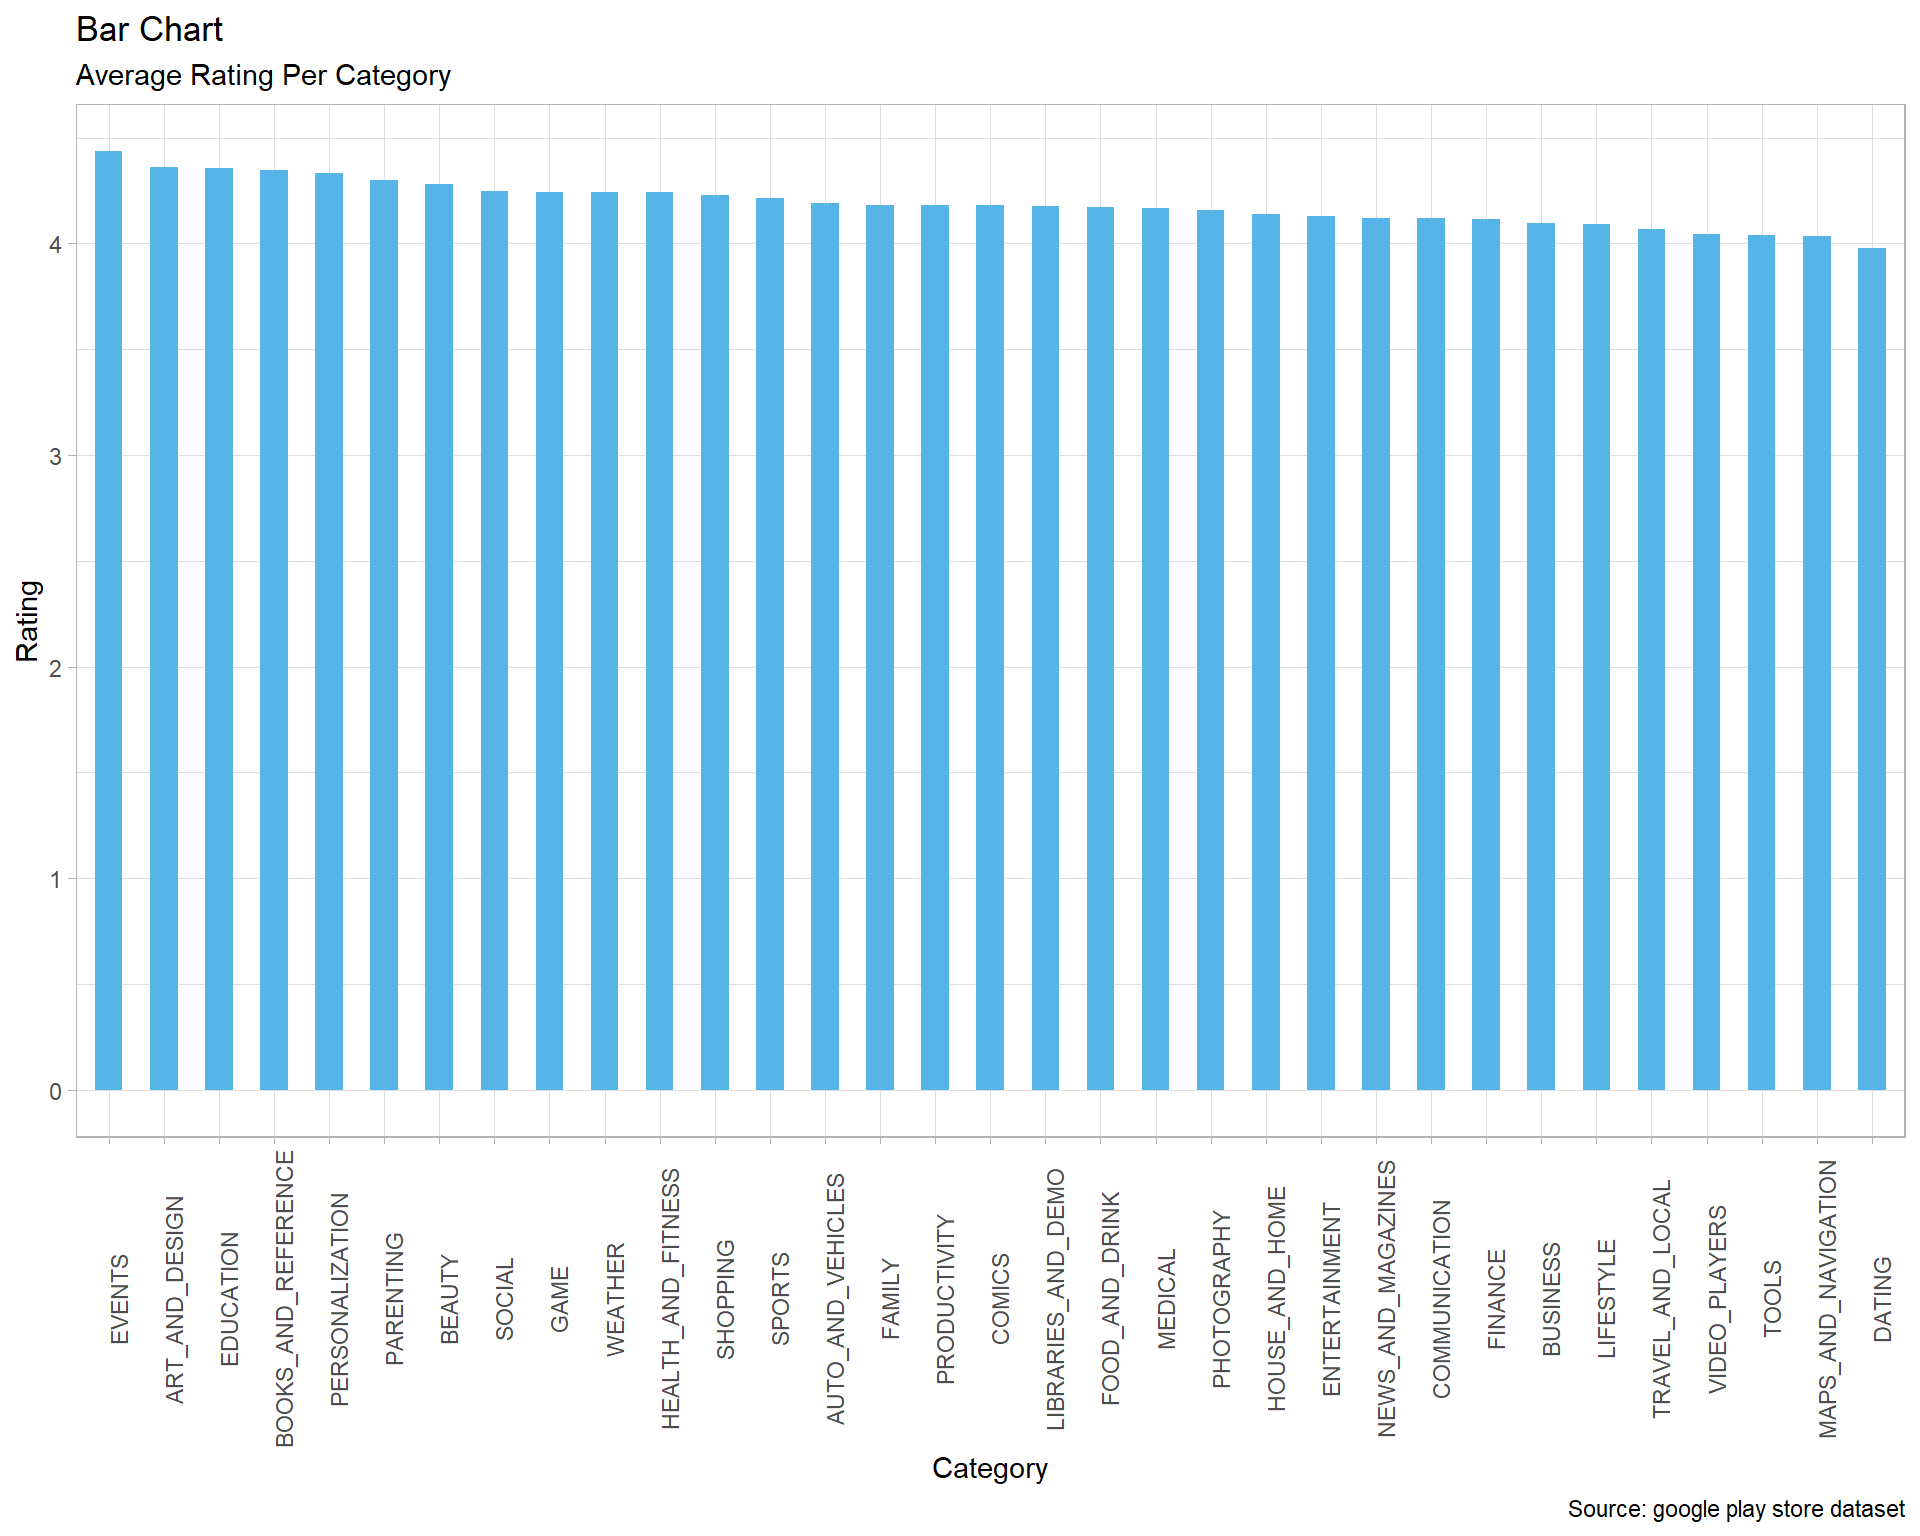
\includegraphics{Group3_final_report_files/figure-latex/avgrating-categoryplot-1.pdf}

\textbf{Finding:} This graph shows that the average rating per category
is not very different. Still the ``EVENTS'' category has the highest
average rating, and ``DATING'' category has the least average rating.

\hypertarget{size-and-rating}{%
\subsubsection{Size and rating}\label{size-and-rating}}

Size is an important aspect, and we want to see the relationship between
size and rating of an application.
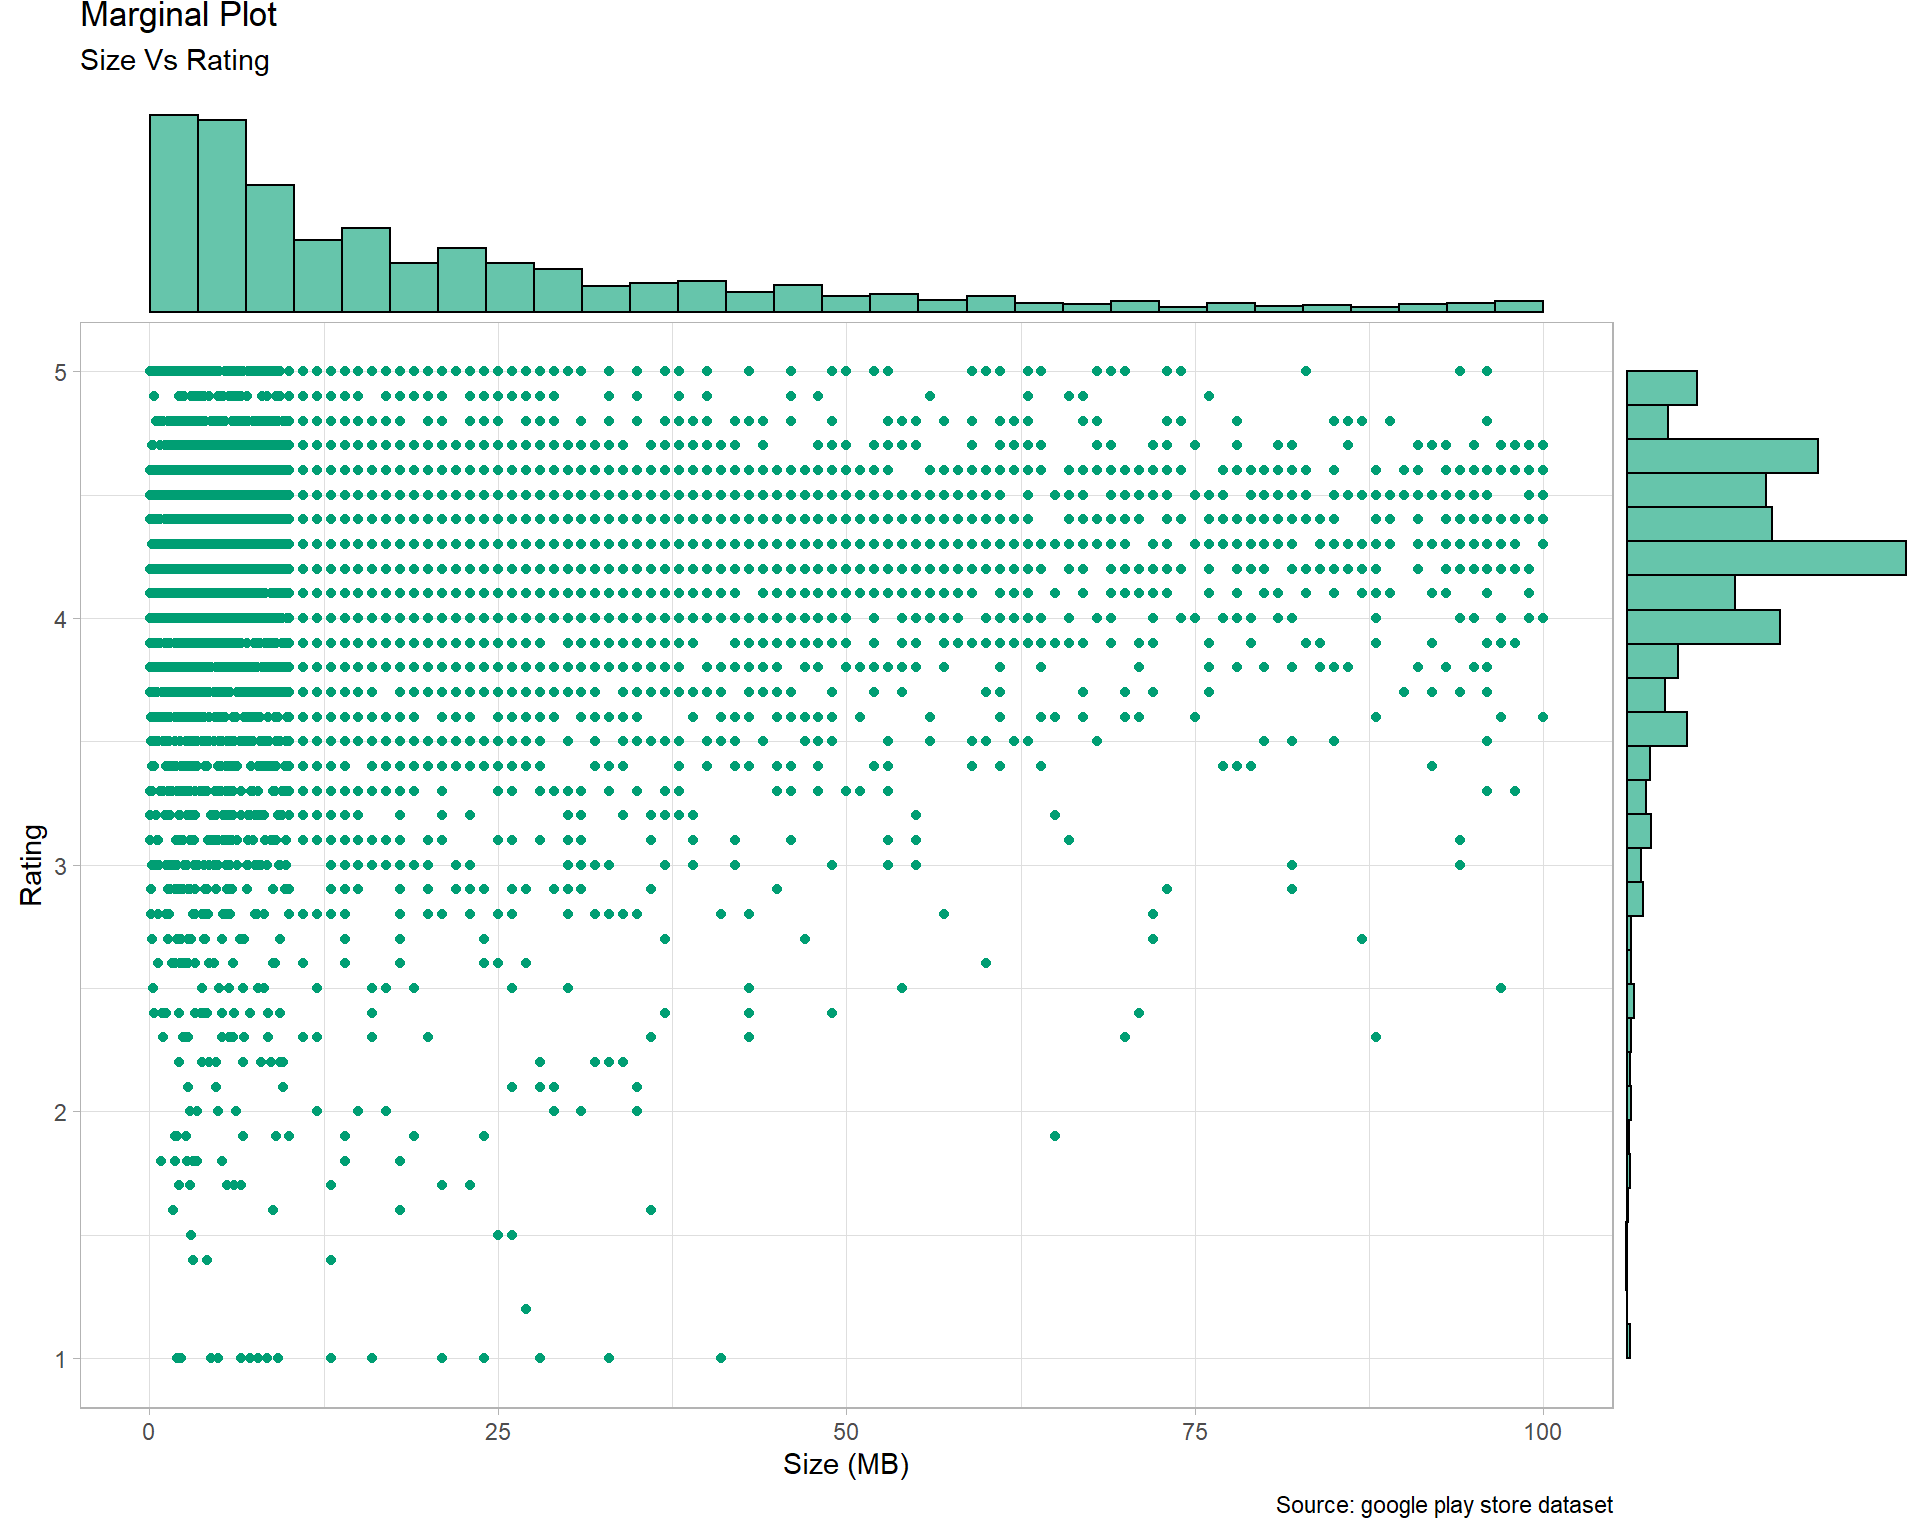
\includegraphics{Group3_final_report_files/figure-latex/size-rating-plot-1.pdf}

\textbf{Finding:} We can see that majority of applications with their
sizes under 25 MB, have a good rating(4).

\hypertarget{installs-column-in-depth}{%
\subsection{Installs column in depth}\label{installs-column-in-depth}}

\hypertarget{number-of-installs-per-category}{%
\subsubsection{Number of installs per
category}\label{number-of-installs-per-category}}

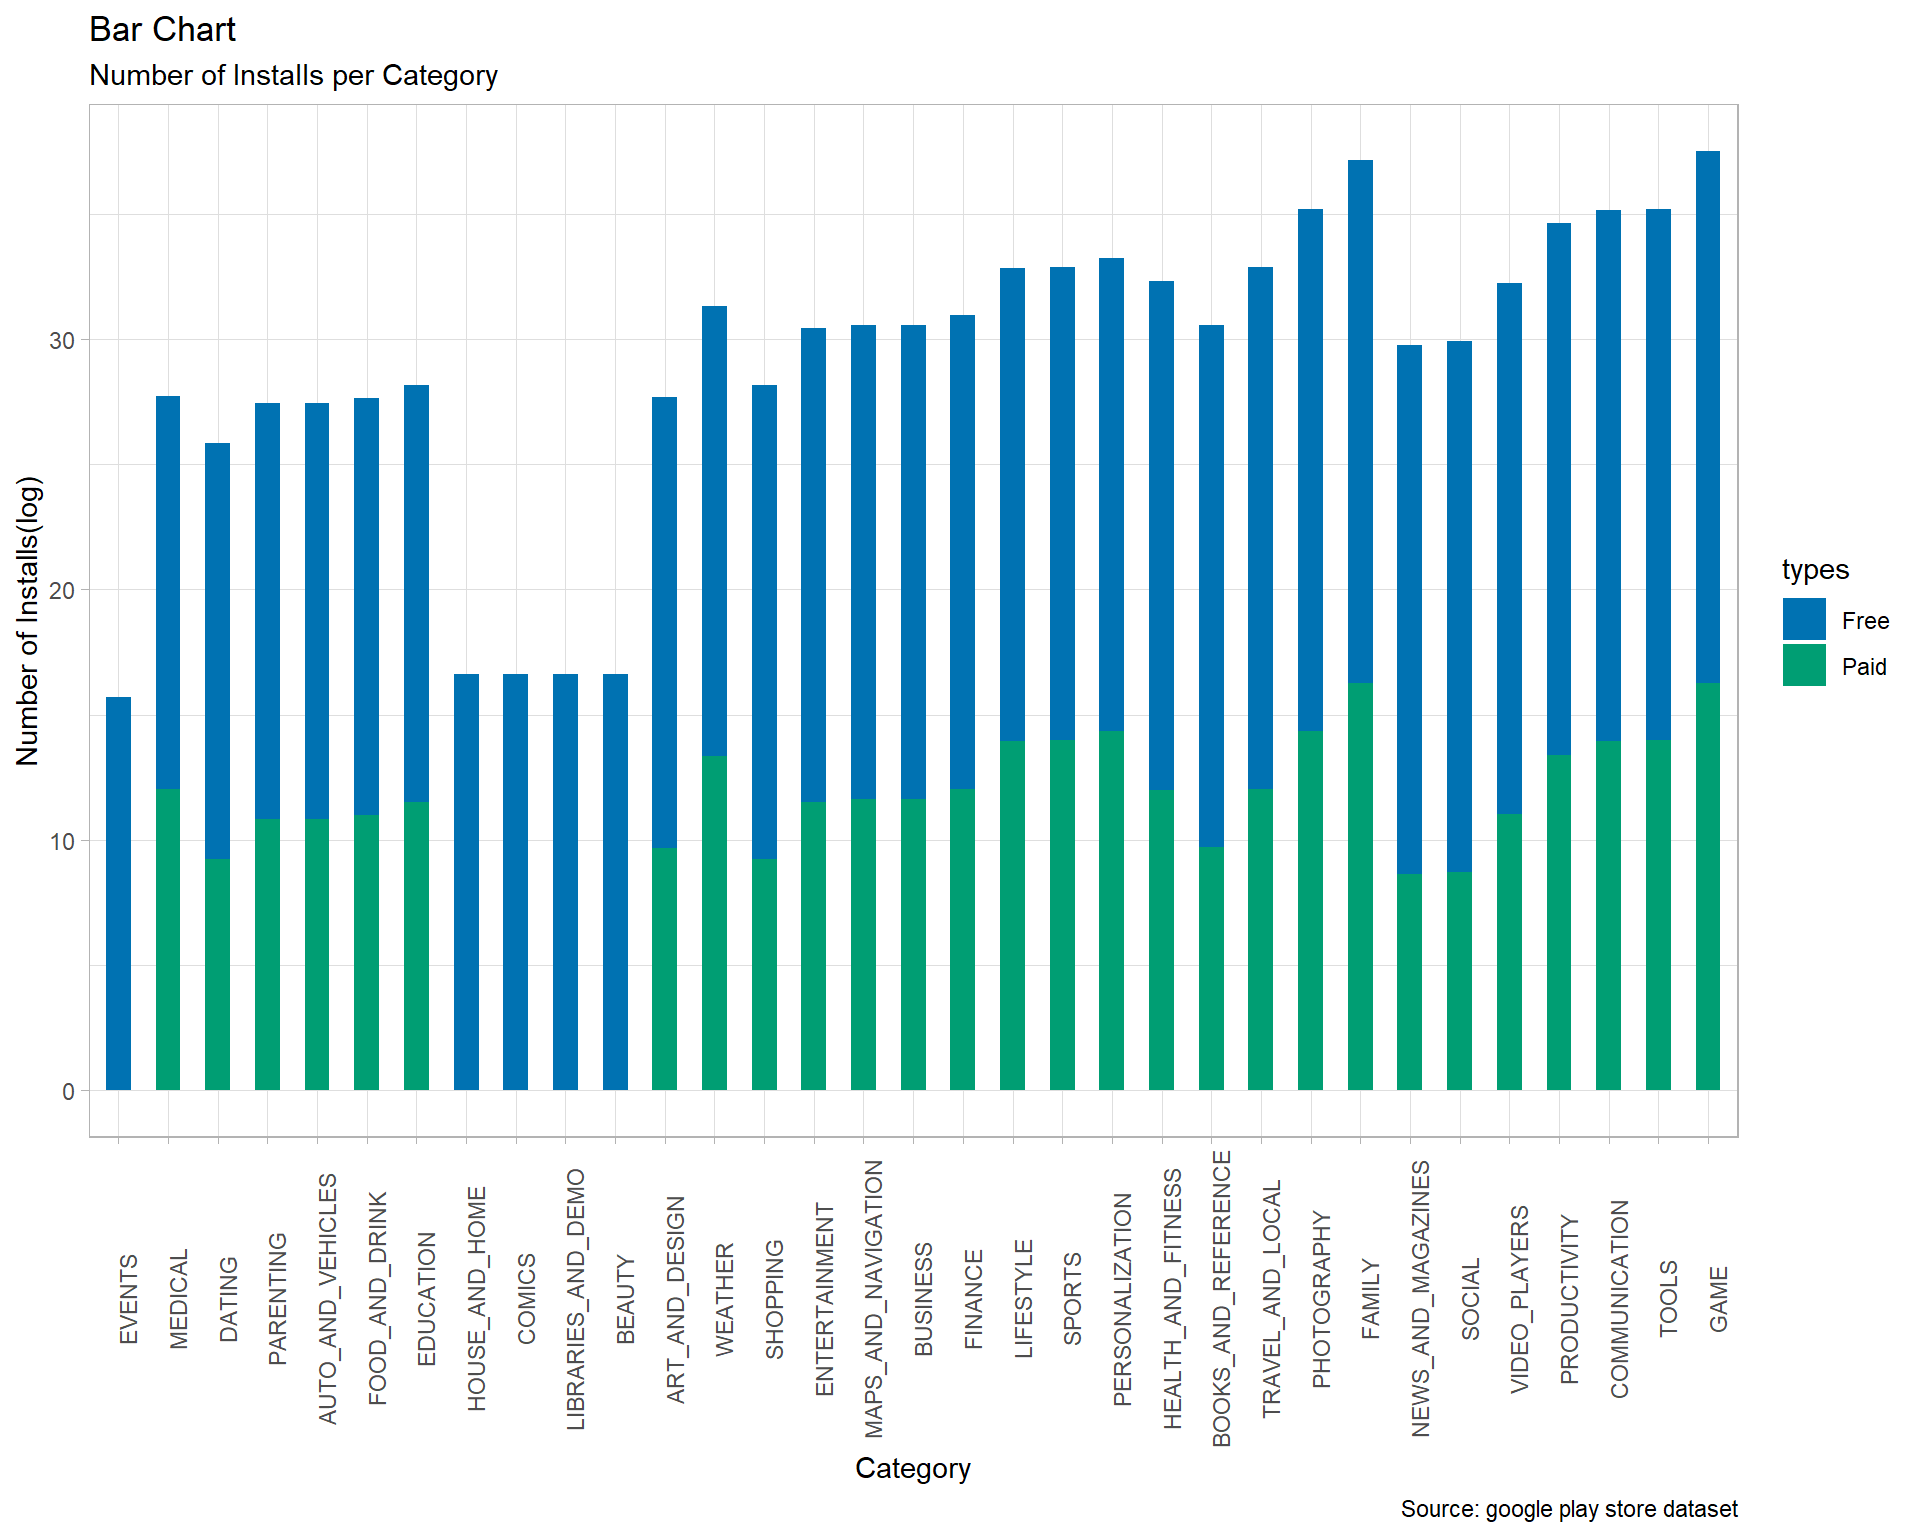
\includegraphics{Group3_final_report_files/figure-latex/installs-percategory-1.pdf}

\textbf{Finding:} The graph shows the log of number of installs (the
values of installs varied from 0 to 1 billion) vs CATEGORY. FAMILY and
GAME has the highest number of installs. EVENTS, HOUSE\_AND\_HOME,
COMICS, LIBRARIES\_AND\_DESIGN and BEAUTY have the least number of
installs.

\hypertarget{top-10-installed-categories}{%
\subsubsection{Top 10 installed
categories}\label{top-10-installed-categories}}

Top 10 categories with greatest number of installs.

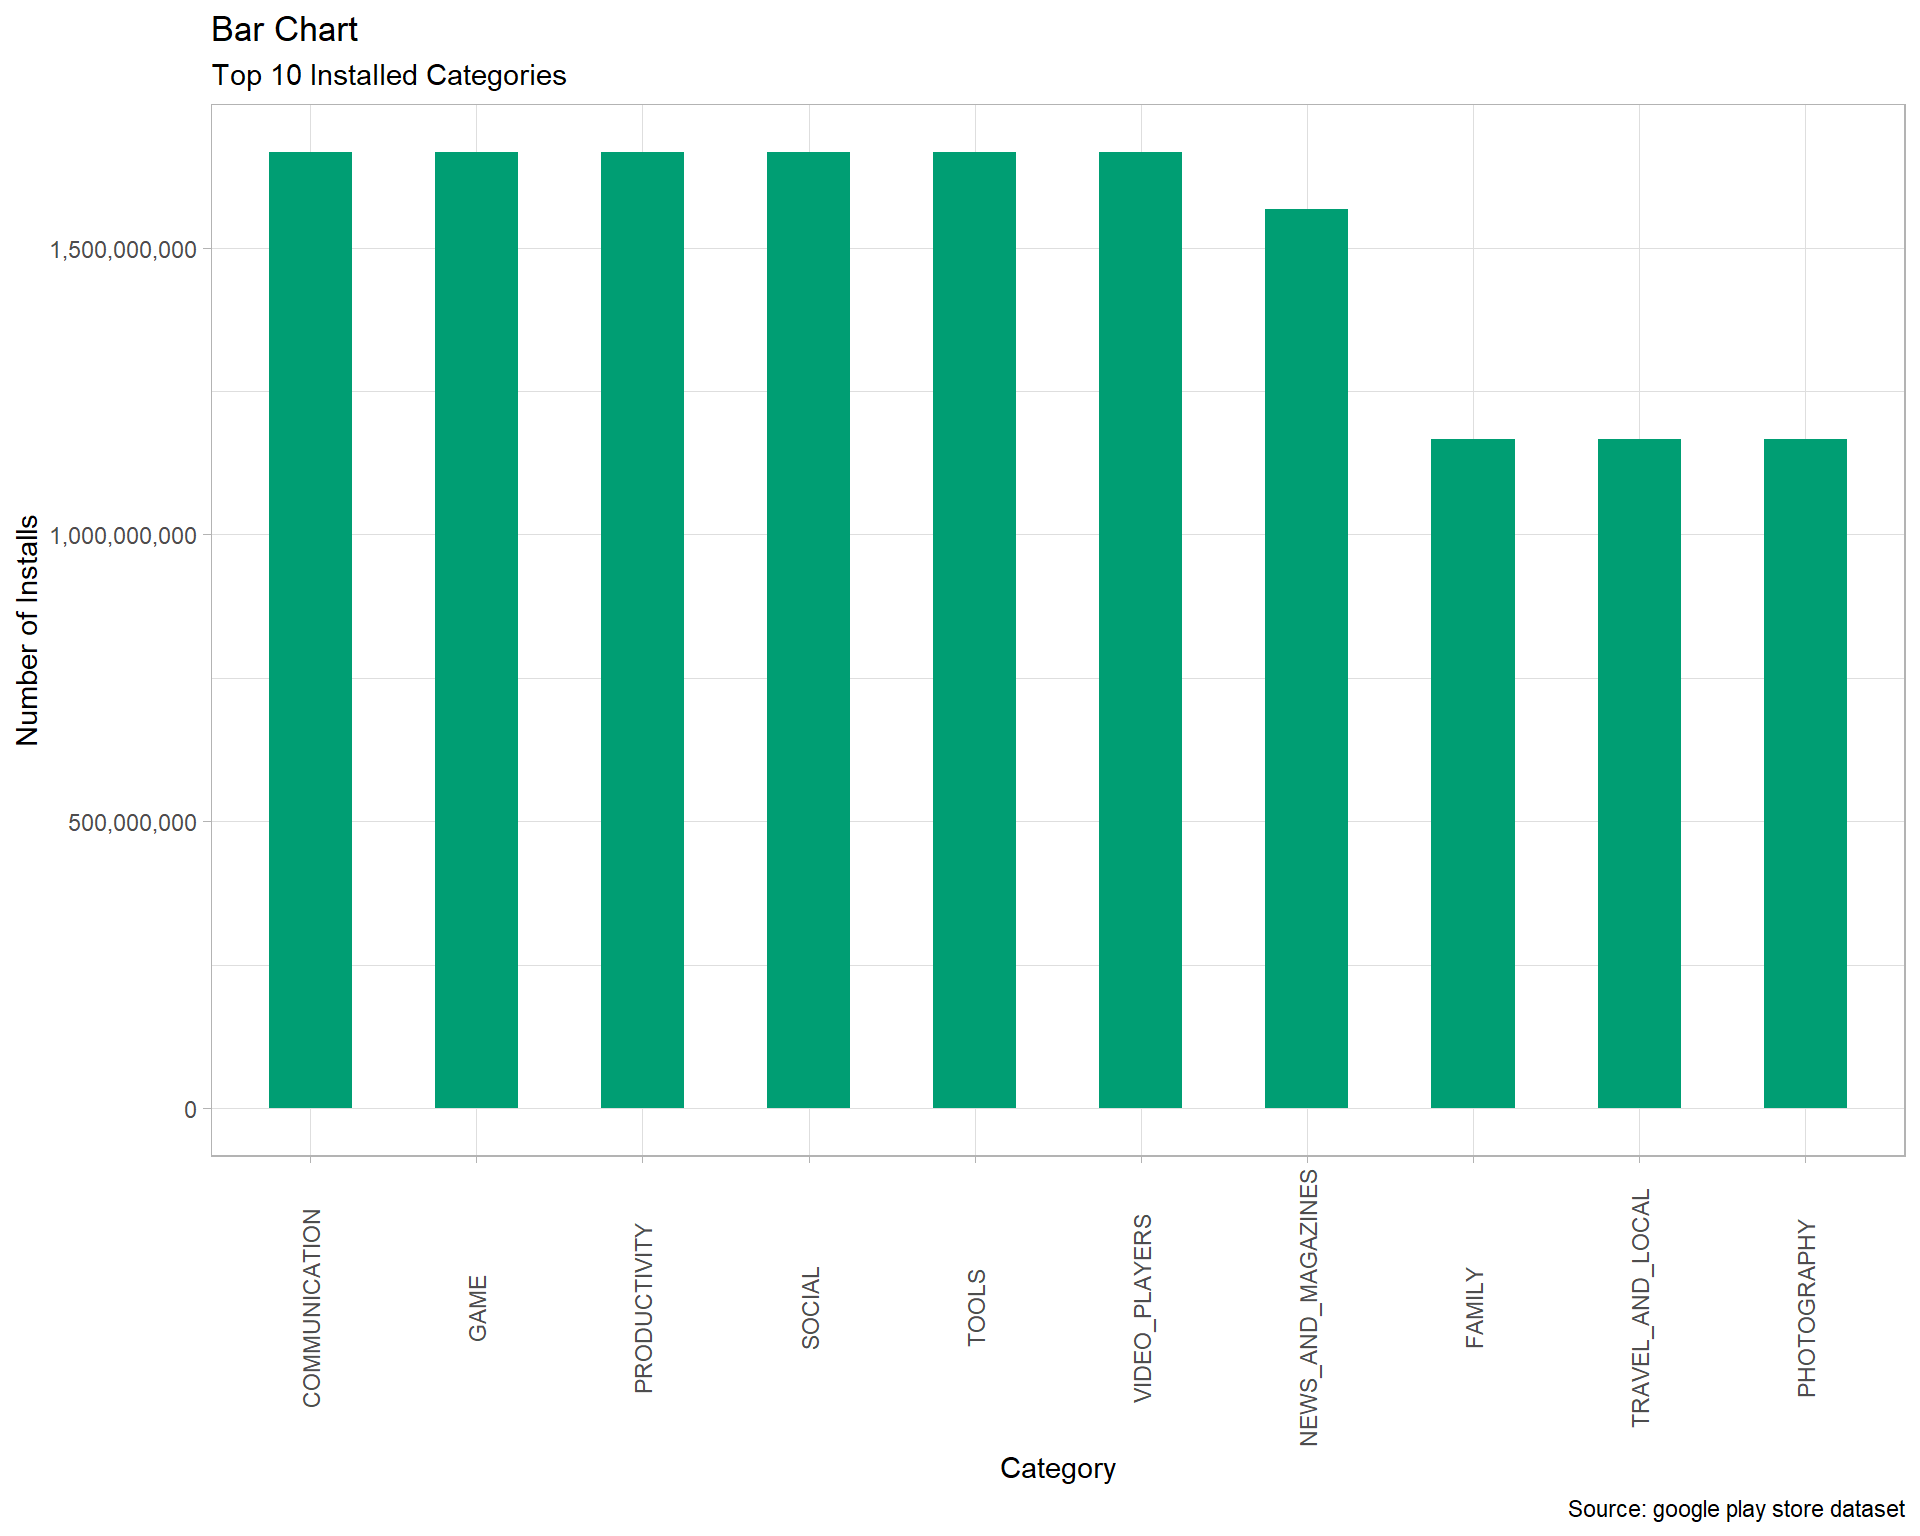
\includegraphics{Group3_final_report_files/figure-latex/top10-installed-categories-1.pdf}

\textbf{Finding:} COMMUNICATION has the highest number of installs.

\hypertarget{least-installed-categories}{%
\subsubsection{10 least installed
categories}\label{least-installed-categories}}

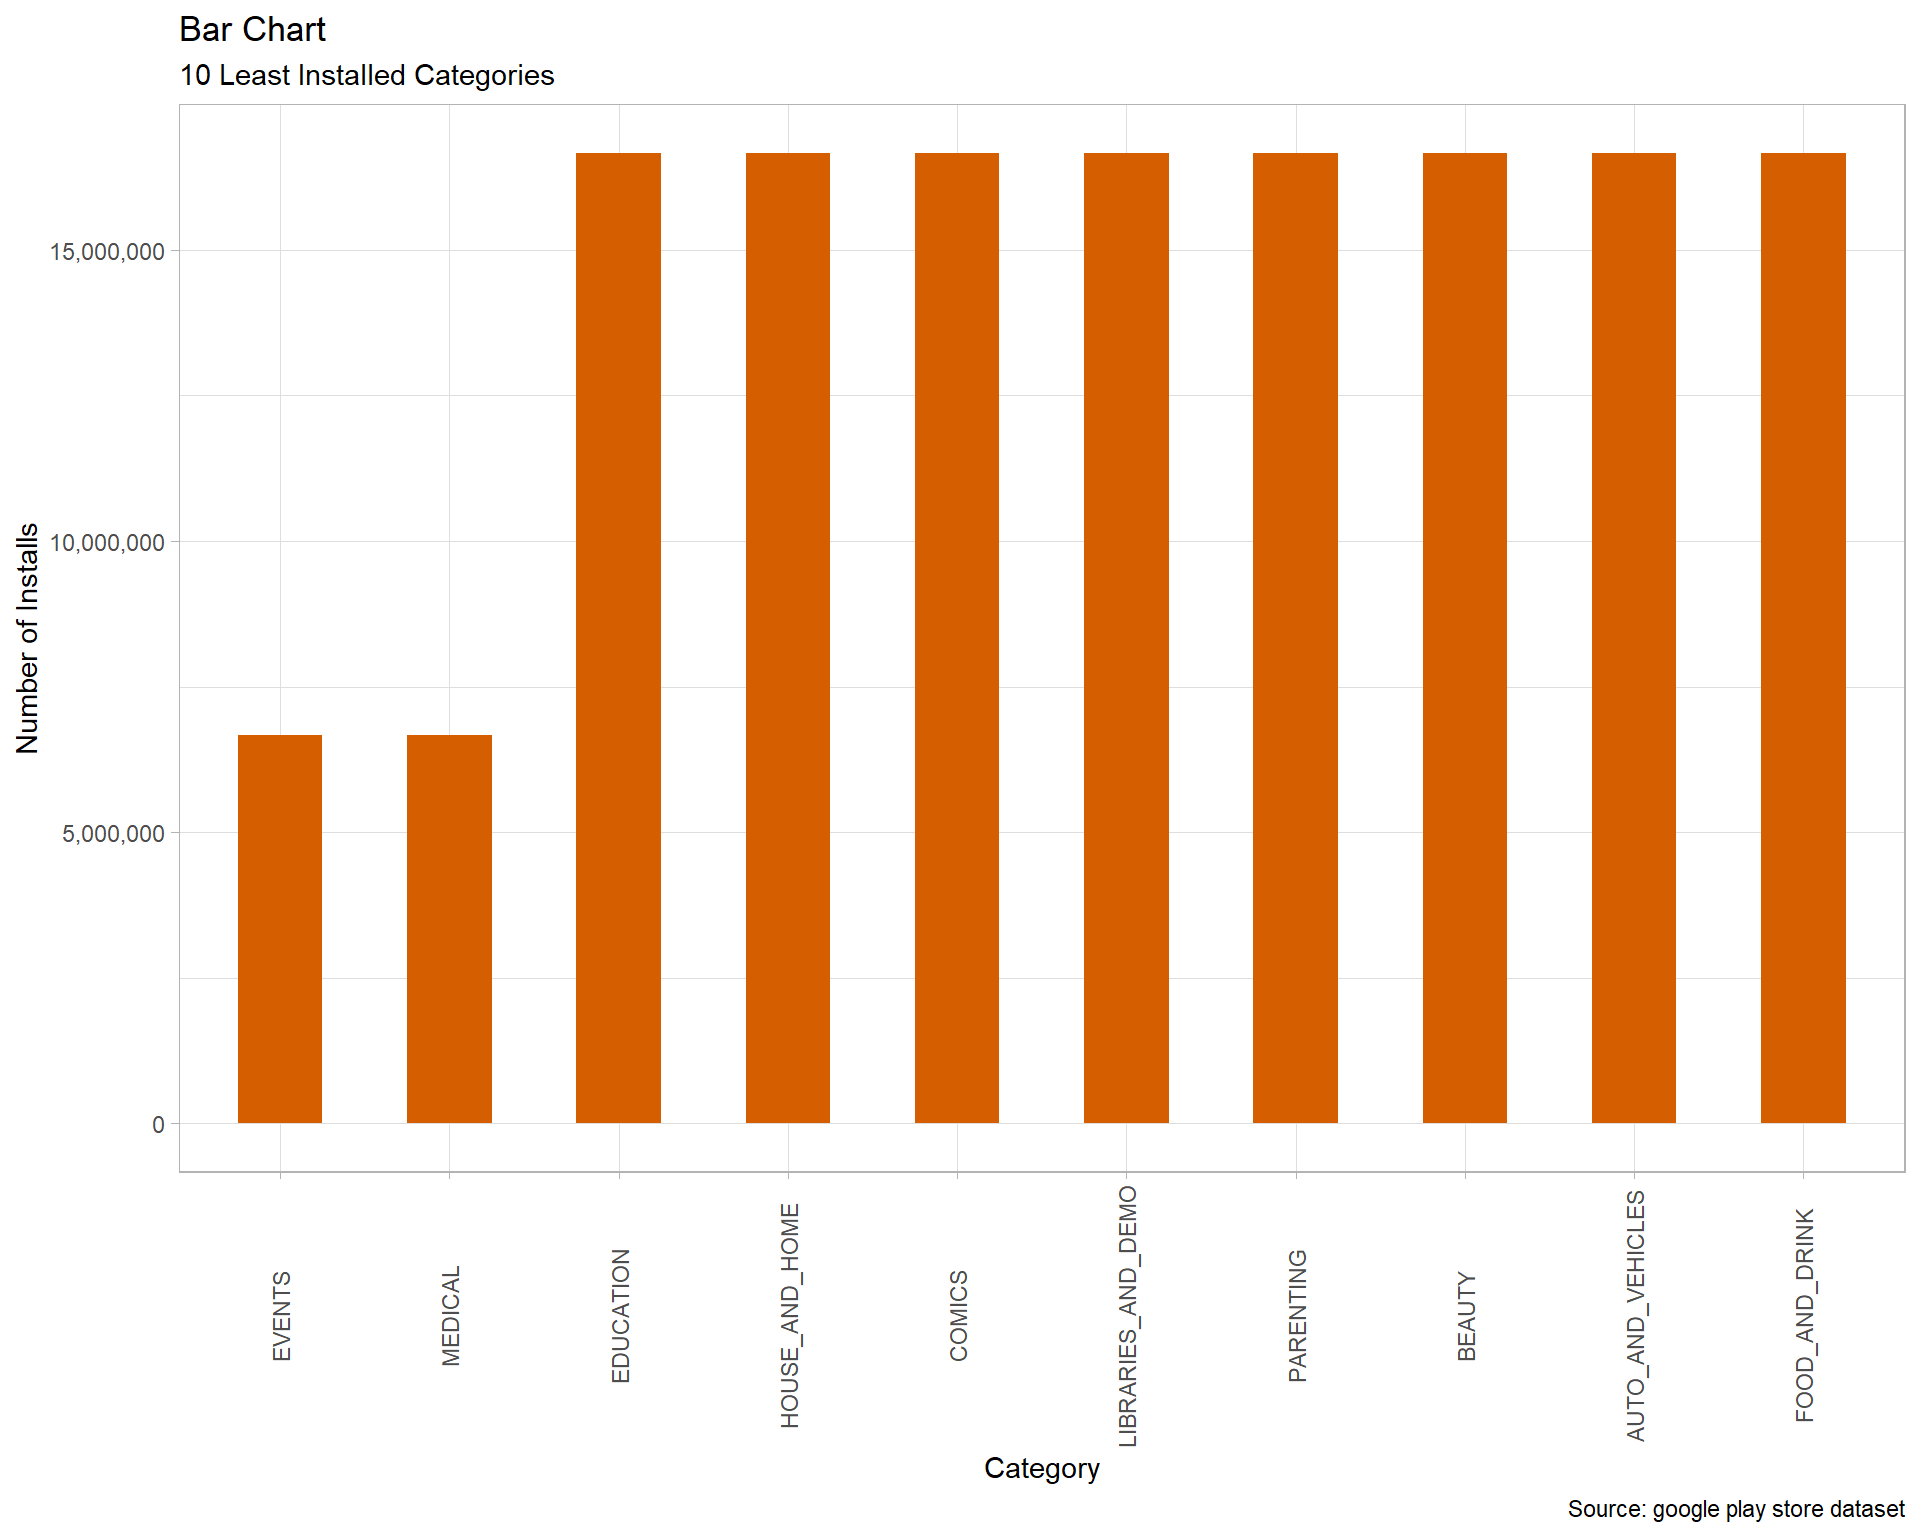
\includegraphics{Group3_final_report_files/figure-latex/bottom10-installed-categories-1.pdf}

\textbf{Finding:} Events has the least number of installed applications.

\hypertarget{top-10-paid-categories}{%
\subsubsection{Top 10 paid Categories}\label{top-10-paid-categories}}

Top 10 categories with the highest number of installs for paid
applications.\\
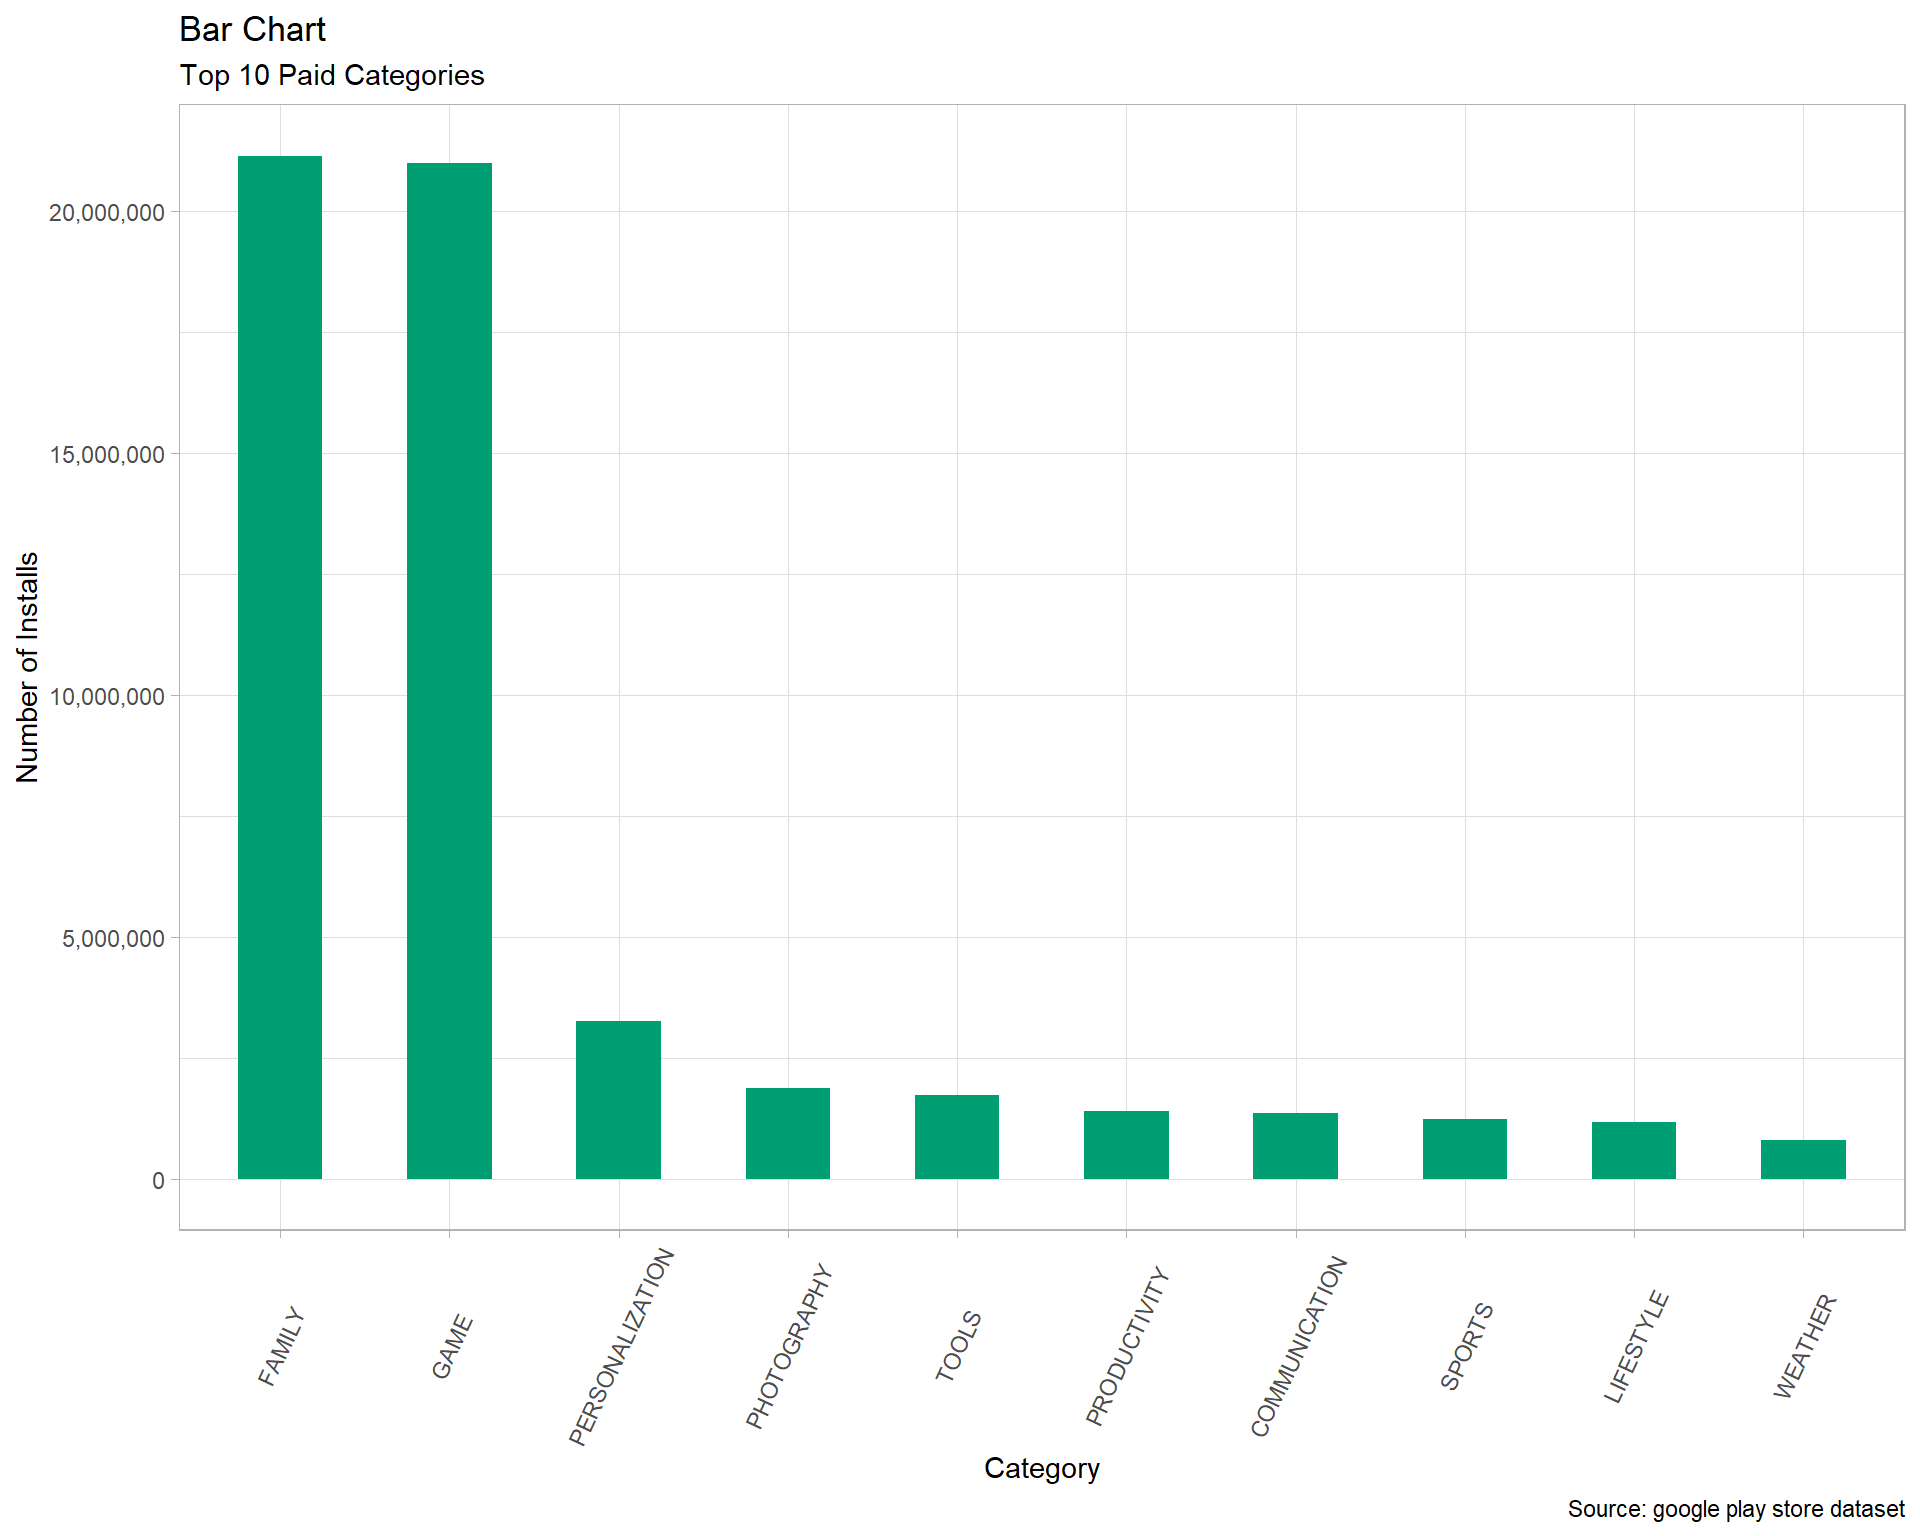
\includegraphics{Group3_final_report_files/figure-latex/top-paid-categories-plot-1.pdf}

\textbf{Finding:} FAMILY and GAME has the greatest number of installs.

\hypertarget{size-vs.-number-of-installs}{%
\subsubsection{Size Vs. number of
installs}\label{size-vs.-number-of-installs}}

Size is an important characteristic of an application. Large
applications might reduce the number of installs, as it reduces to
targeted audience. We can test this by plotting size against installs.
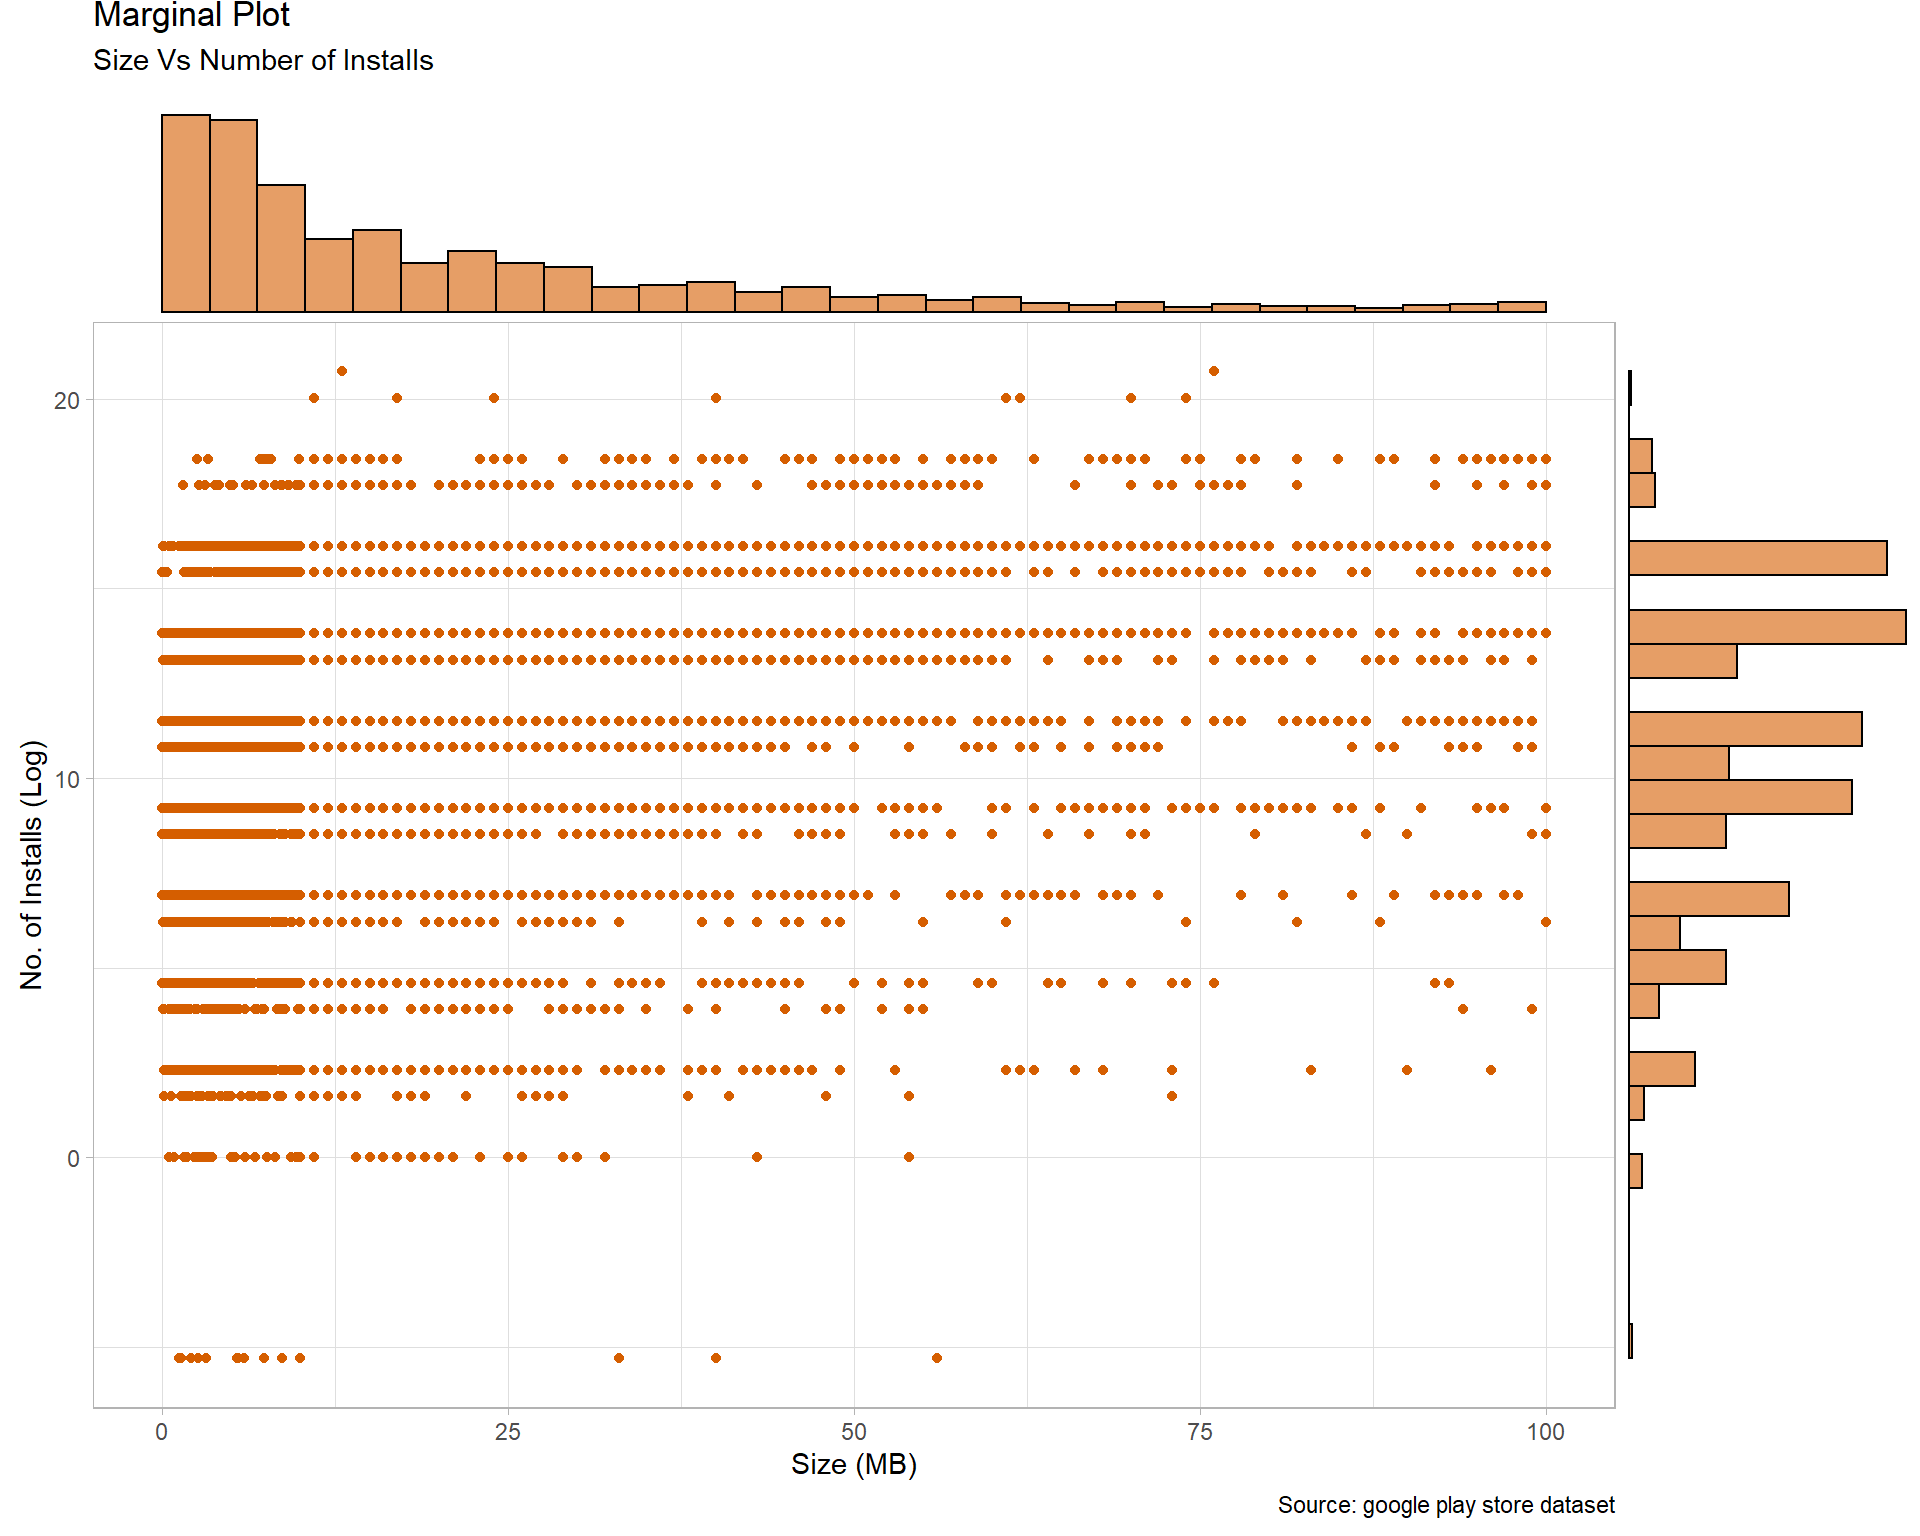
\includegraphics{Group3_final_report_files/figure-latex/size-installs-plot-1.pdf}

\textbf{Finding:} Optimally sized Applications, with sizes between 5MB
and 30MB, gets the greatest number of installs.

\hypertarget{number-of-installs-based-on-support-by-minimum-android-version}{%
\subsubsection{Number of installs based on support by minimum android
version}\label{number-of-installs-based-on-support-by-minimum-android-version}}

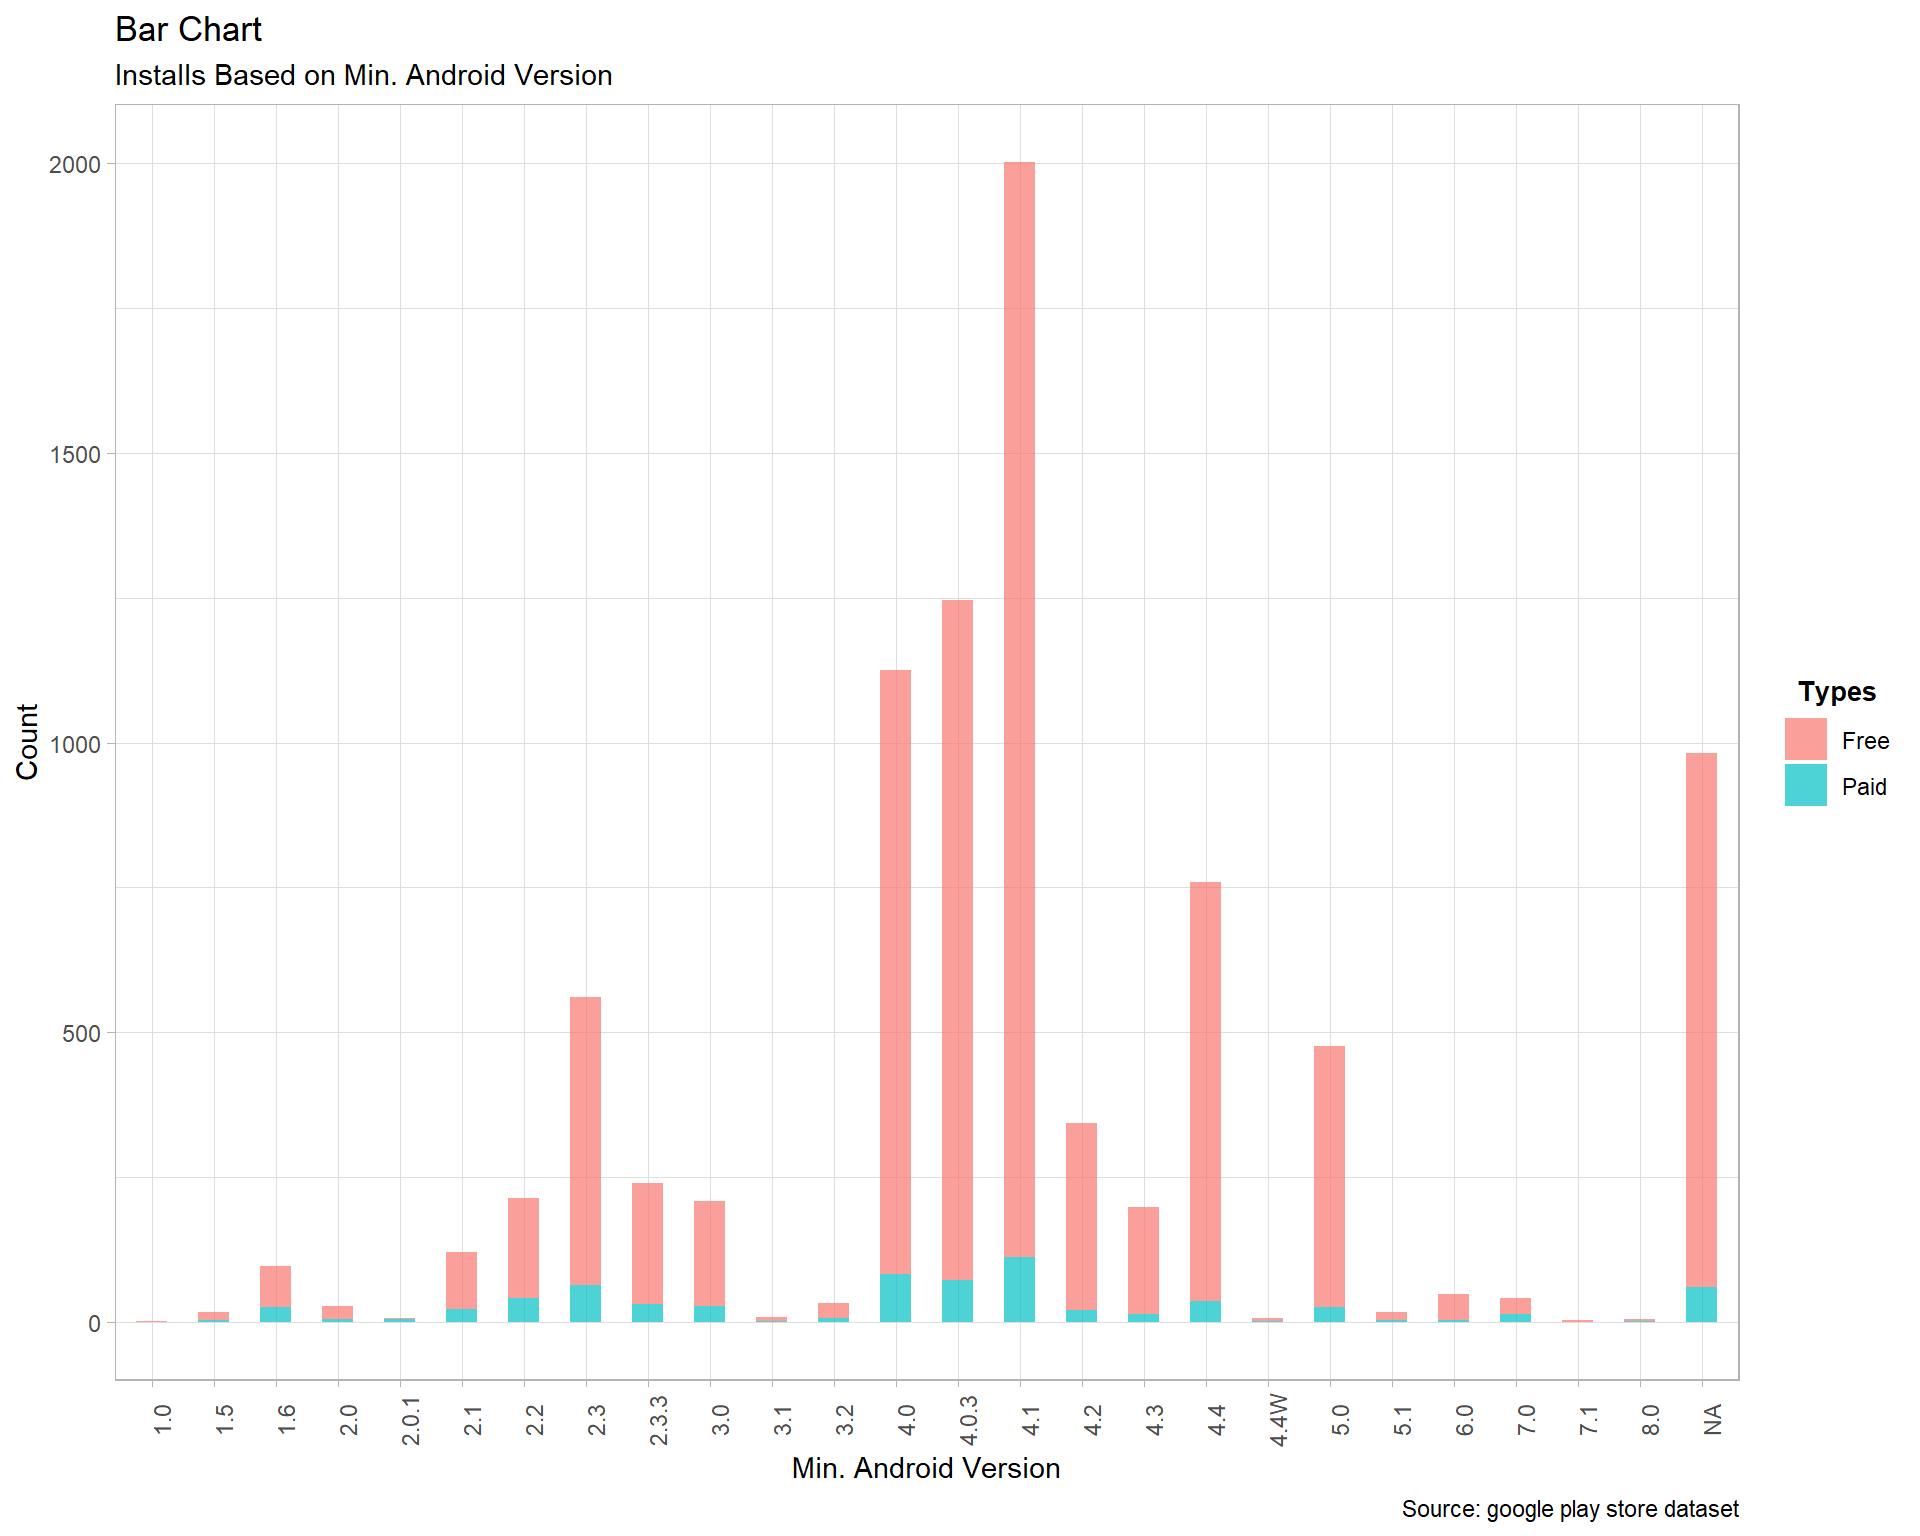
\includegraphics{Group3_final_report_files/figure-latex/android_ver-1.pdf}

\textbf{Finding:} 4.1 android version has the maximum number of
installs.

\hypertarget{conclusion}{%
\section{Conclusion}\label{conclusion}}

\begin{itemize}
\tightlist
\item
  To get most success from an app, it has to have maximum number of
  reviews and maximum number of ratings. These are the other trends we
  found:

  \begin{itemize}
  \tightlist
  \item
    Apps should atleast support 4.1 android version or more to
    succeed.This is expected because the majority of users have smart
    phones with constant android updates.\\
  \item
    They have high chances of success if the genre is family, game,
    communication or productivity apps whereas food\_and\_drink,
    auto\_vehicles categories have very low probability to succeed.\\
  \item
    The apps which are be free have huge success rates however there are
    a few exceptions to this.\\
  \item
    Apps should be optimally sized between 5MB and 30MB.
  \end{itemize}
\end{itemize}

\hypertarget{future-work-models}{%
\section{Future work (models)}\label{future-work-models}}

\hypertarget{what-are-we-trying-to-achieve-thesishypothesis}{%
\subsection{What are we trying to achieve
(thesis/hypothesis)}\label{what-are-we-trying-to-achieve-thesishypothesis}}

The dataset we have contains information about 10000 apps dated till
2018. With the dataset, we plan on using Linear Regression Model,
Recursive Partitioning Model and Random Forest to perform predictive
analysis. We want to answer the following hypothesis:

\begin{enumerate}
\def\labelenumi{\arabic{enumi})}
\tightlist
\item
  Find similarities in apps that make it to the top of Play Store.
  Factors contributing to the success of applications.
\item
  Can we predict rating of apps based on other parameters such as number
  of reviews or the size of an app?
\end{enumerate}

To answer these questions, we will be exploring all the variables of
this dataset to find if there's any relationship between rating and
other variables. We intend to find out which of these variables will
play the most important role in predicting rating.

\hypertarget{why-is-this-importantinteresting}{%
\subsection{Why is this
important/interesting?}\label{why-is-this-importantinteresting}}

Before we started this project, we took part in a competition called
game-jam {[}12{]} where we built a game,we had an idea of launching it
on Google Play Store.We then thought it would be interesting to see
currents trends in the market and to do a detailed analysis to get more
insights to the following questions:\\
1.Factors that influence the success of an app,\\
2.Which categories are highly installed\\
3.What are the most famous applications and do they have any trends in
common like number of installs, number of reviews, size or
android-version? and etc

These analysis inturn will aid the developer community to build
successful apps targeting a specific audience.

\hypertarget{how-are-we-going-to-test-the-hypothesis}{%
\subsection{How are we going to test the
hypothesis?}\label{how-are-we-going-to-test-the-hypothesis}}

Since the dataset is dated till 2018. We are thinking to test it by
comparing the predictions of our model with the 2019 dataset or the
latest dataset.

\hypertarget{any-challenges-that-we-might-encounter}{%
\subsection{Any challenges that we might
encounter}\label{any-challenges-that-we-might-encounter}}

There is a lot of useful information that could have given us more
insight into the Play Store market e.g.~Demographic data could have
offered insights into the rating and number of installs of apps, with
respect to different regions, different cultures and different trends
popular to specific age groups. Also, it would have been interesting to
see how different global trends affect the usage of the app, for
instance, the current pandemic ``covid-19'' has called for quarantine
across the globe and many people, markets and other companies are
relying on smart phones and virtual connections, this will heavily
increase the use of many applications, thus deviating from the general
trend.

\hypertarget{model}{%
\section{Model}\label{model}}

\begin{itemize}
\item
  Our main goal is to predict rating of an app based on different
  parameters. Our EDA confirms that variables like number of installs,
  number of reviews, category of the app and the type of app (paid/free)
  highly affect the rating of an app.
\item
  In this section, we try to fit both explanatory and predictive models.
  We used the cross validation technique to select the best fitting
  model for our dataset and lastly, we test the models by predicting
  ratings for a dummy app.
\end{itemize}

\hypertarget{correlation-using-pearson-method}{%
\subsection{Correlation using Pearson
method}\label{correlation-using-pearson-method}}

Before creating a model, we will investigate the correlation between
different variables to help select the exploratory variables.

\begin{verbatim}
## 
##  Pearson's product-moment correlation
## 
## data:  clean_play_store$installs and clean_play_store$rating
## t = 3.6459, df = 8194, p-value = 0.0002681
## alternative hypothesis: true correlation is not equal to 0
## 95 percent confidence interval:
##  0.01861078 0.06184077
## sample estimates:
##        cor 
## 0.04024461
\end{verbatim}

\begin{verbatim}
## 
##  Pearson's product-moment correlation
## 
## data:  log10(clean_play_store$installs)^2 and clean_play_store$rating
## t = 10.376, df = 8194, p-value < 2.2e-16
## alternative hypothesis: true correlation is not equal to 0
## 95 percent confidence interval:
##  0.0924570 0.1351958
## sample estimates:
##       cor 
## 0.1138791
\end{verbatim}

\begin{itemize}
\tightlist
\item
  \textbf{Correlation coefficient between rating and installs}: The
  correlation coefficient is 0.0402. Using the square of log transform
  of the installs variable increased the correlation coefficient to
  0.1138. This indicates that there is a slight positive relation
  between the variables which can also be observed in the graphs (given
  in the next section) where the blue line indicates the best fitted
  Local Regression model and the red line shows a Recursive Partitioning
  model.
\end{itemize}

\begin{verbatim}
## 
##  Pearson's product-moment correlation
## 
## data:  clean_play_store$reviews and clean_play_store$rating
## t = 5.0001, df = 8194, p-value = 5.849e-07
## alternative hypothesis: true correlation is not equal to 0
## 95 percent confidence interval:
##  0.03354294 0.07671138
## sample estimates:
##        cor 
## 0.05515293
\end{verbatim}

\begin{verbatim}
## 
##  Pearson's product-moment correlation
## 
## data:  log10(clean_play_store$reviews)^2 and clean_play_store$rating
## t = 18.775, df = 8194, p-value < 2.2e-16
## alternative hypothesis: true correlation is not equal to 0
## 95 percent confidence interval:
##  0.1822407 0.2237556
## sample estimates:
##       cor 
## 0.2030894
\end{verbatim}

\begin{itemize}
\tightlist
\item
  \textbf{Correlation coefficient between rating and reviews}: The
  correlation coefficient is 0.05515. Using the square of log transform
  of the installs variable increased the correlation coefficient to
  .20308.
\end{itemize}

\hypertarget{explanatorydescriptive-modeling}{%
\subsection{Explanatory/Descriptive
modeling}\label{explanatorydescriptive-modeling}}

\begin{itemize}
\tightlist
\item
  The following models are used:
\item
  Linear Regression Model
\item
  Local Regression Model
\item
  Recursive Partitioning Model
\end{itemize}

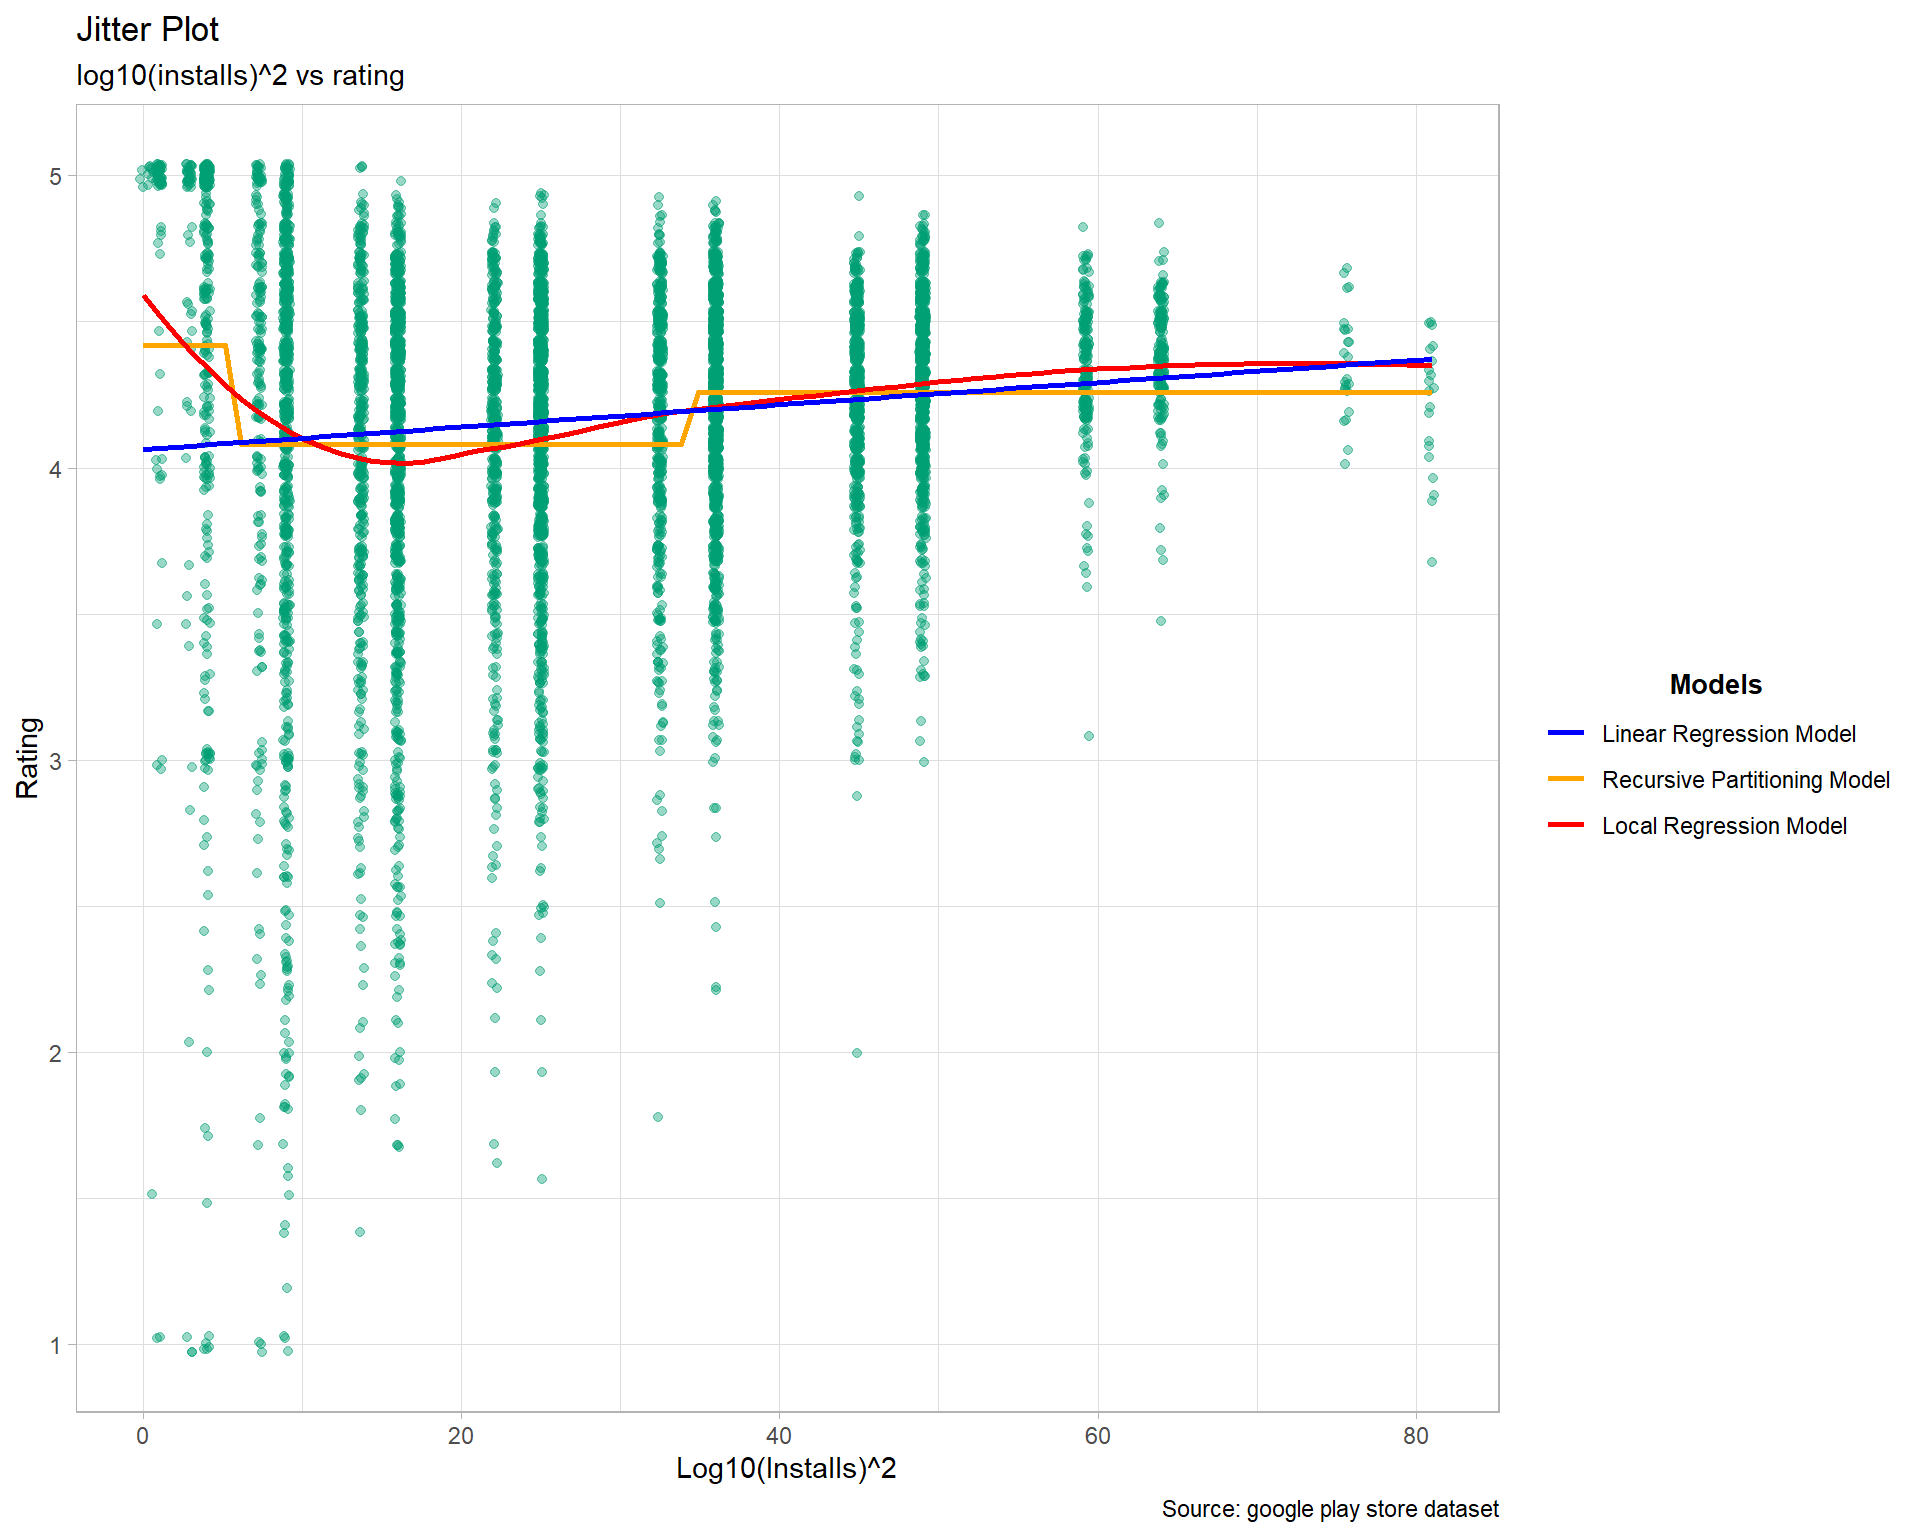
\includegraphics{Group3_final_report_files/figure-latex/descriptive_modeling_1-1.pdf}
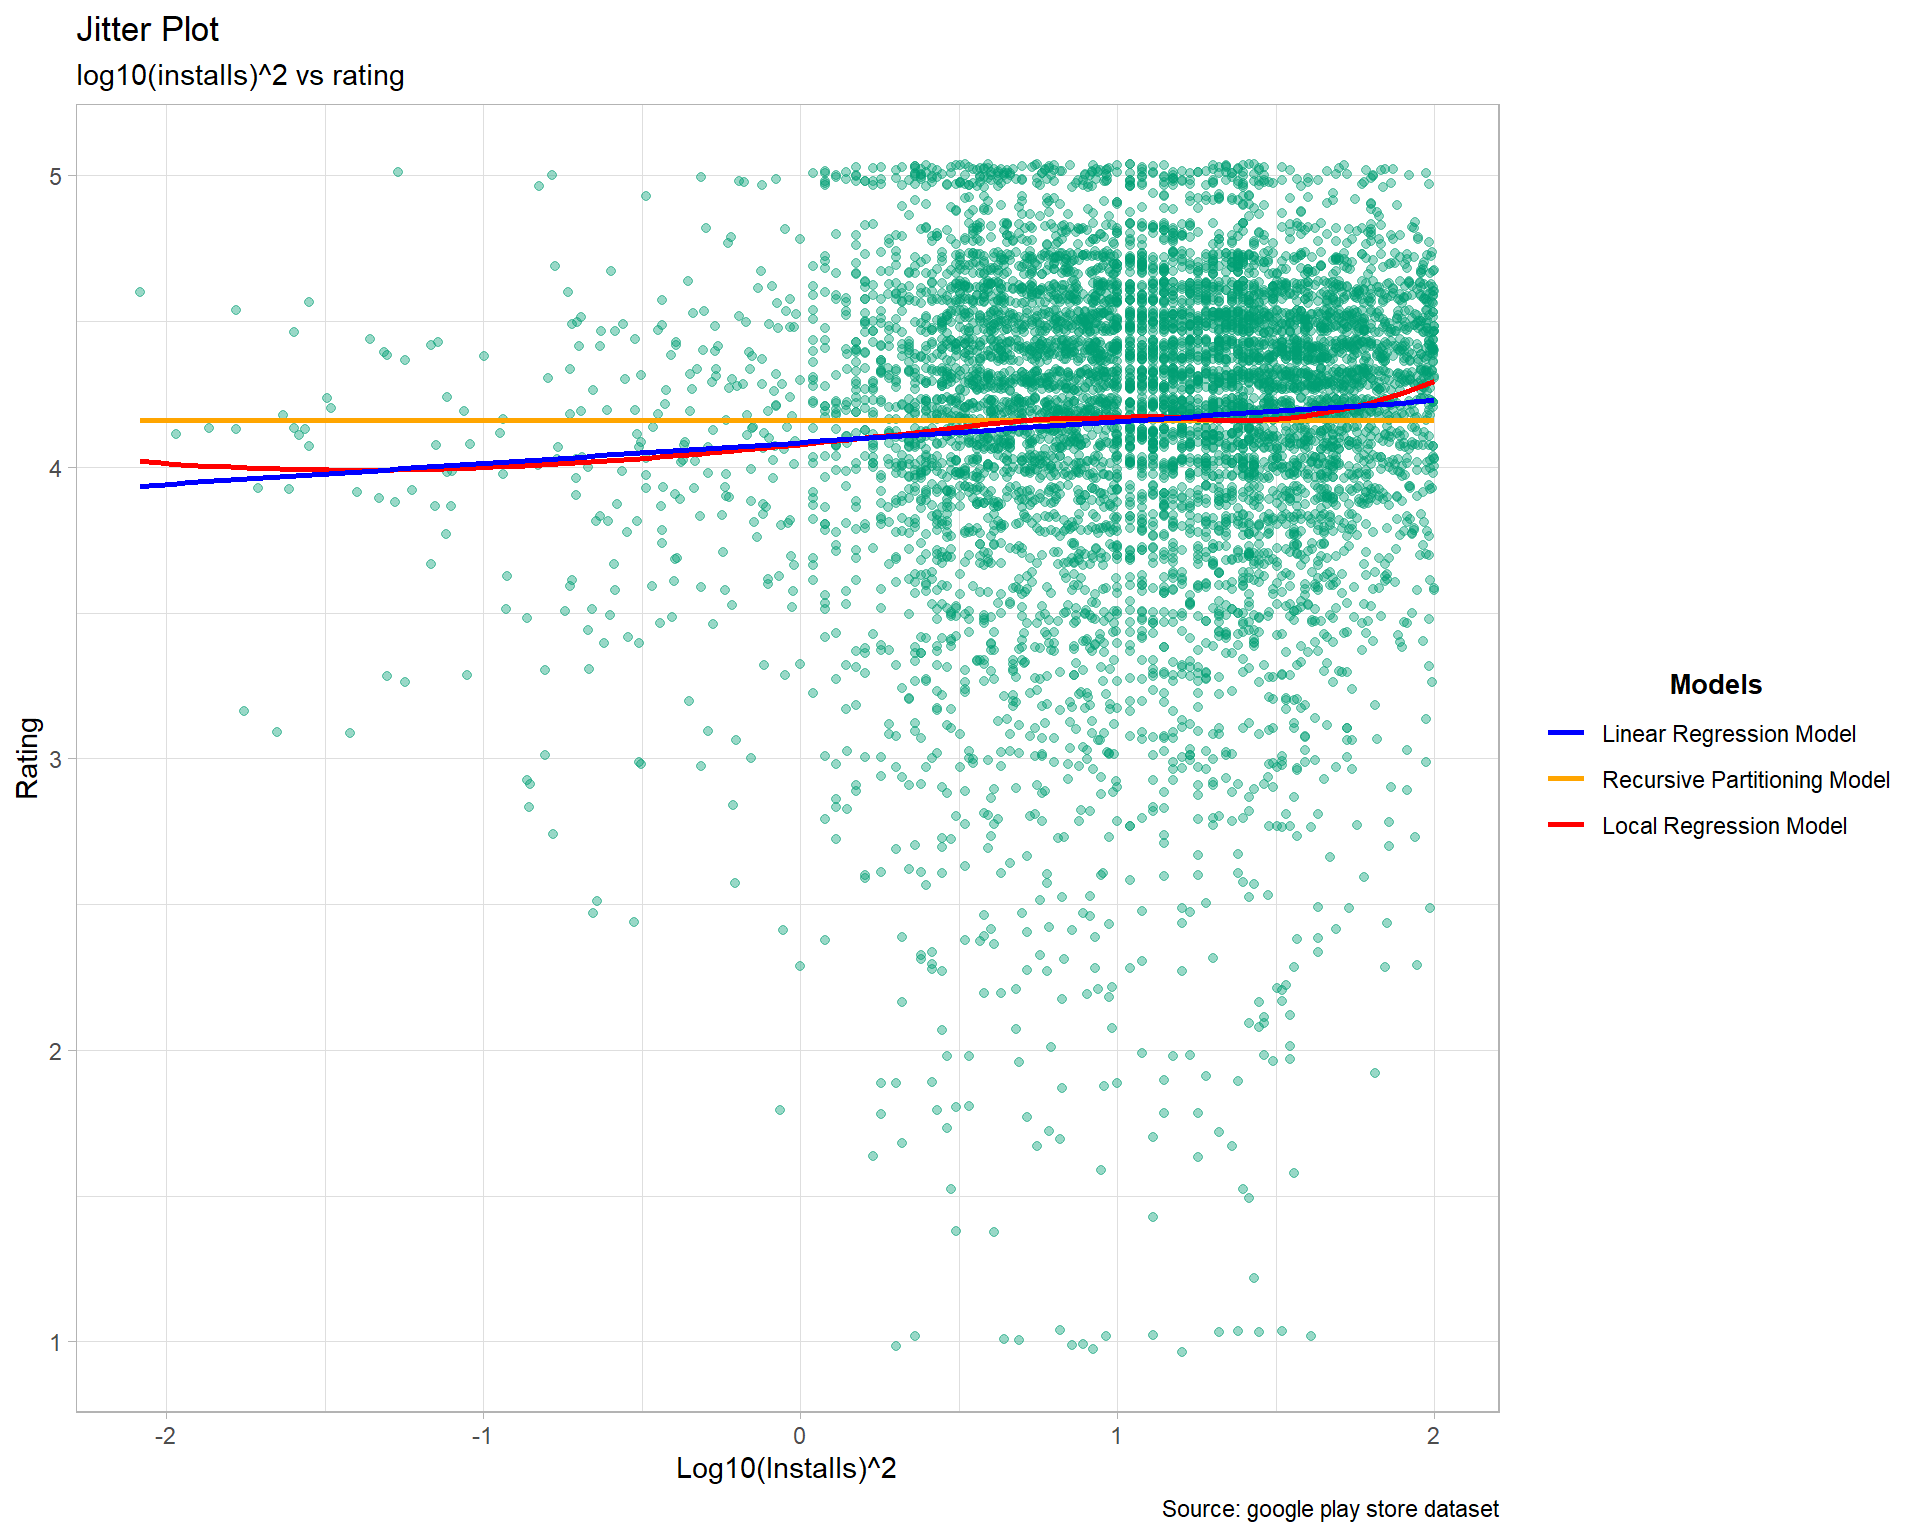
\includegraphics{Group3_final_report_files/figure-latex/descriptive_modeling_1-2.pdf}
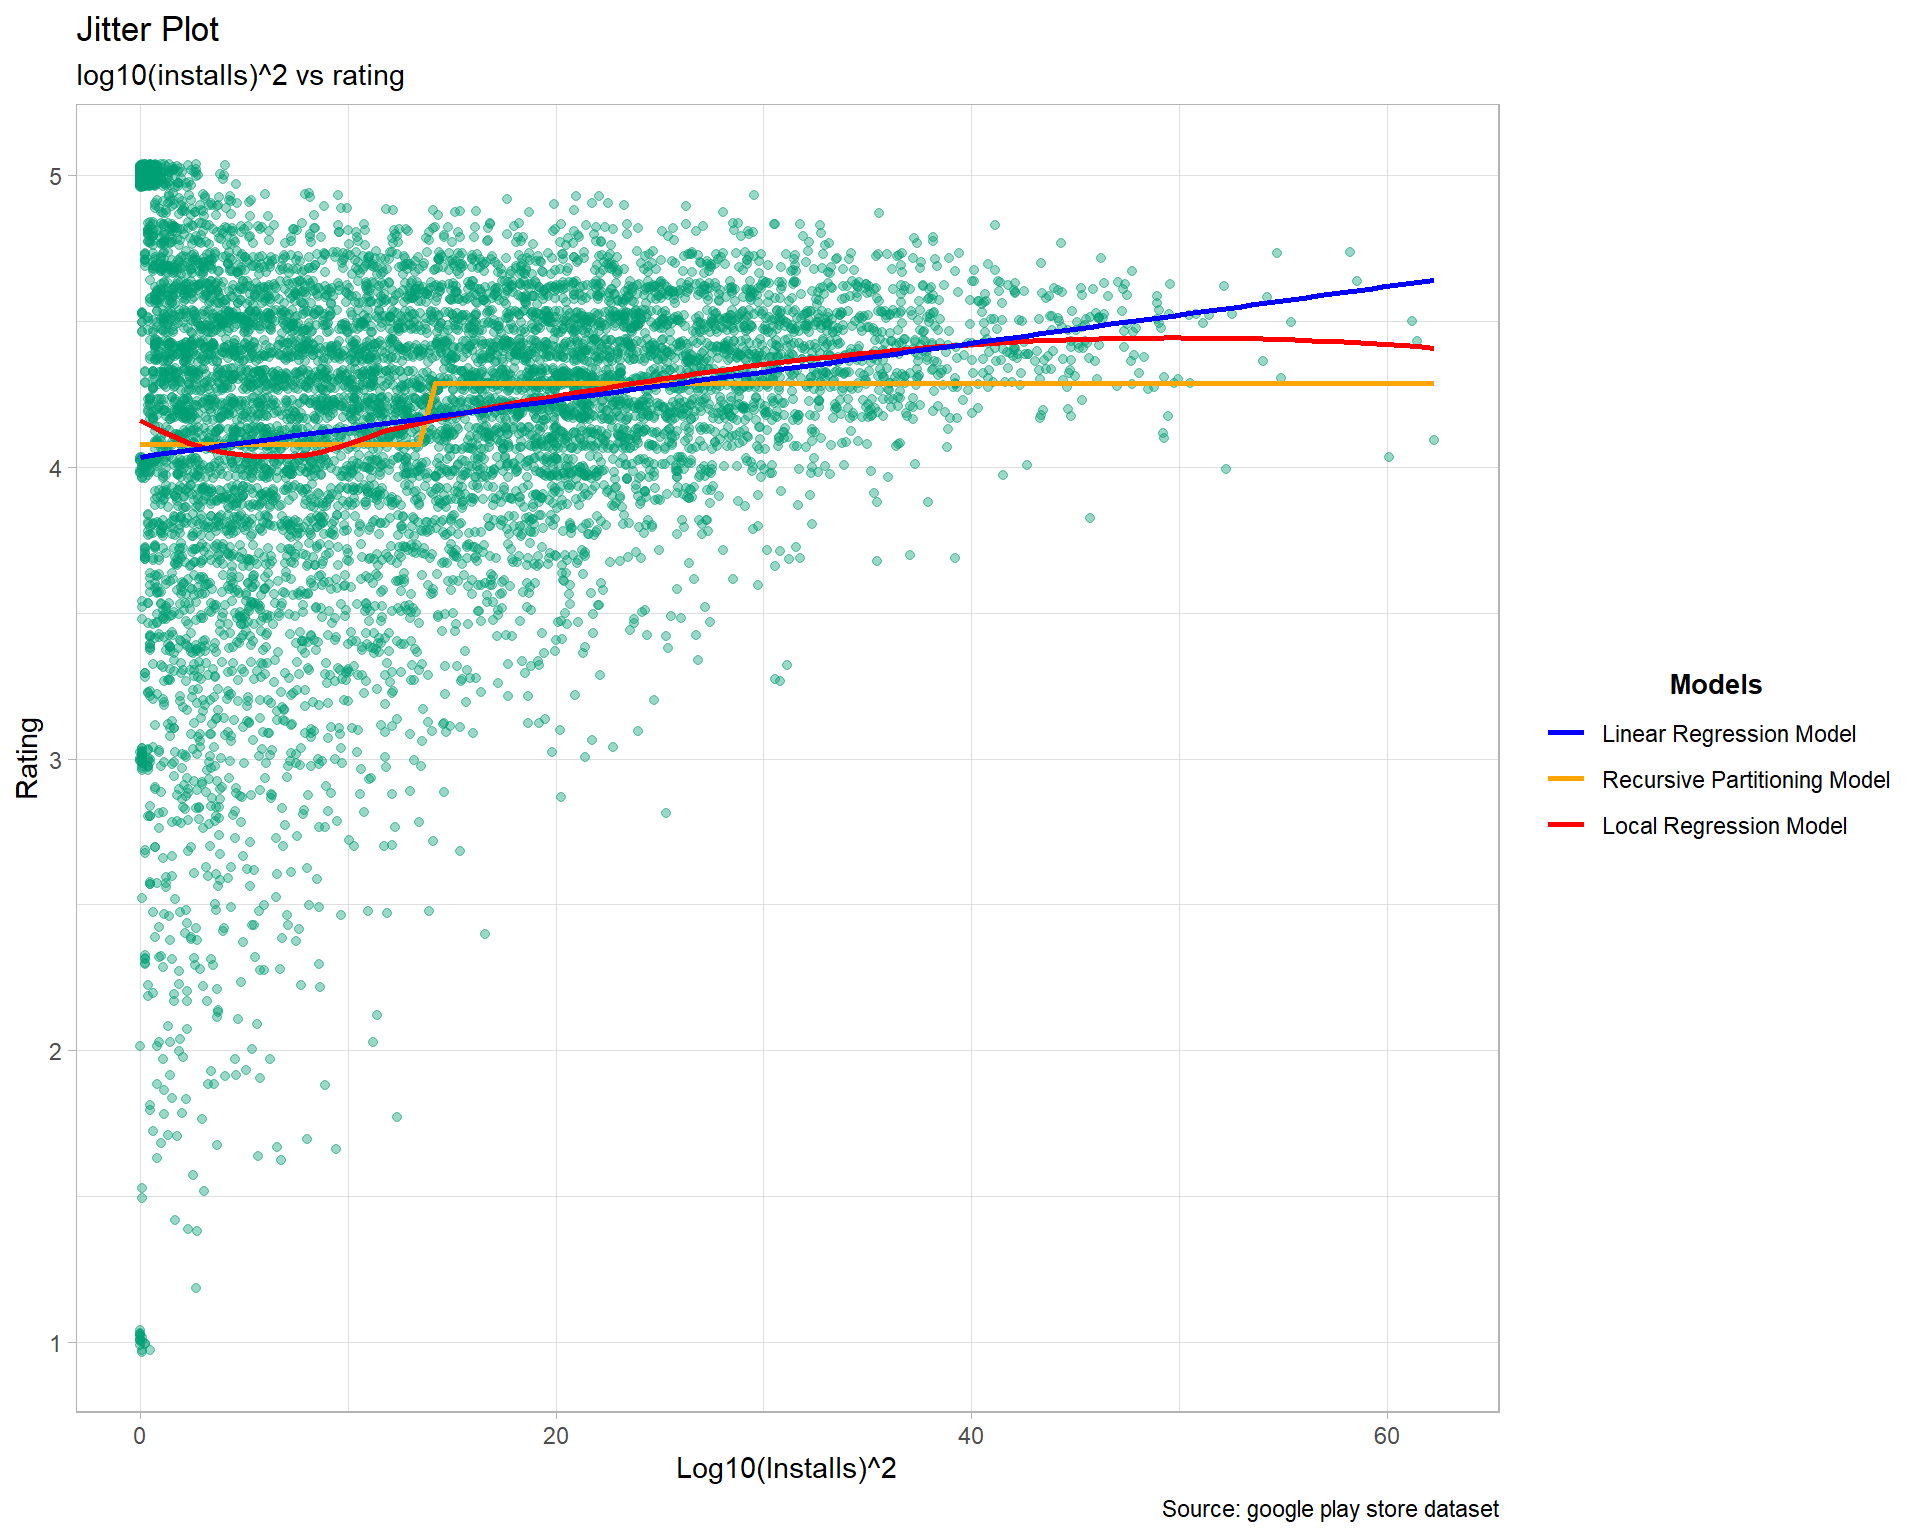
\includegraphics{Group3_final_report_files/figure-latex/descriptive_modeling_1-3.pdf}
The above graphs show the fitted Linear Regression model, Local
Regression model and Recursive Partitioning model for predicting rating
using number of installs, size of the app and number of reviews
variables.

\hypertarget{explanatorydescriptive-modeling-cont.}{%
\subsection{Explanatory/Descriptive modeling
(cont.)}\label{explanatorydescriptive-modeling-cont.}}

Continuing with our explanatory modeling we will fit a model for rating
vs installs given taking into consideration whether the app is Free or
Paid. We have also calculated sum of square residuals, R-Square value
and Root Mean Square Error for the model.

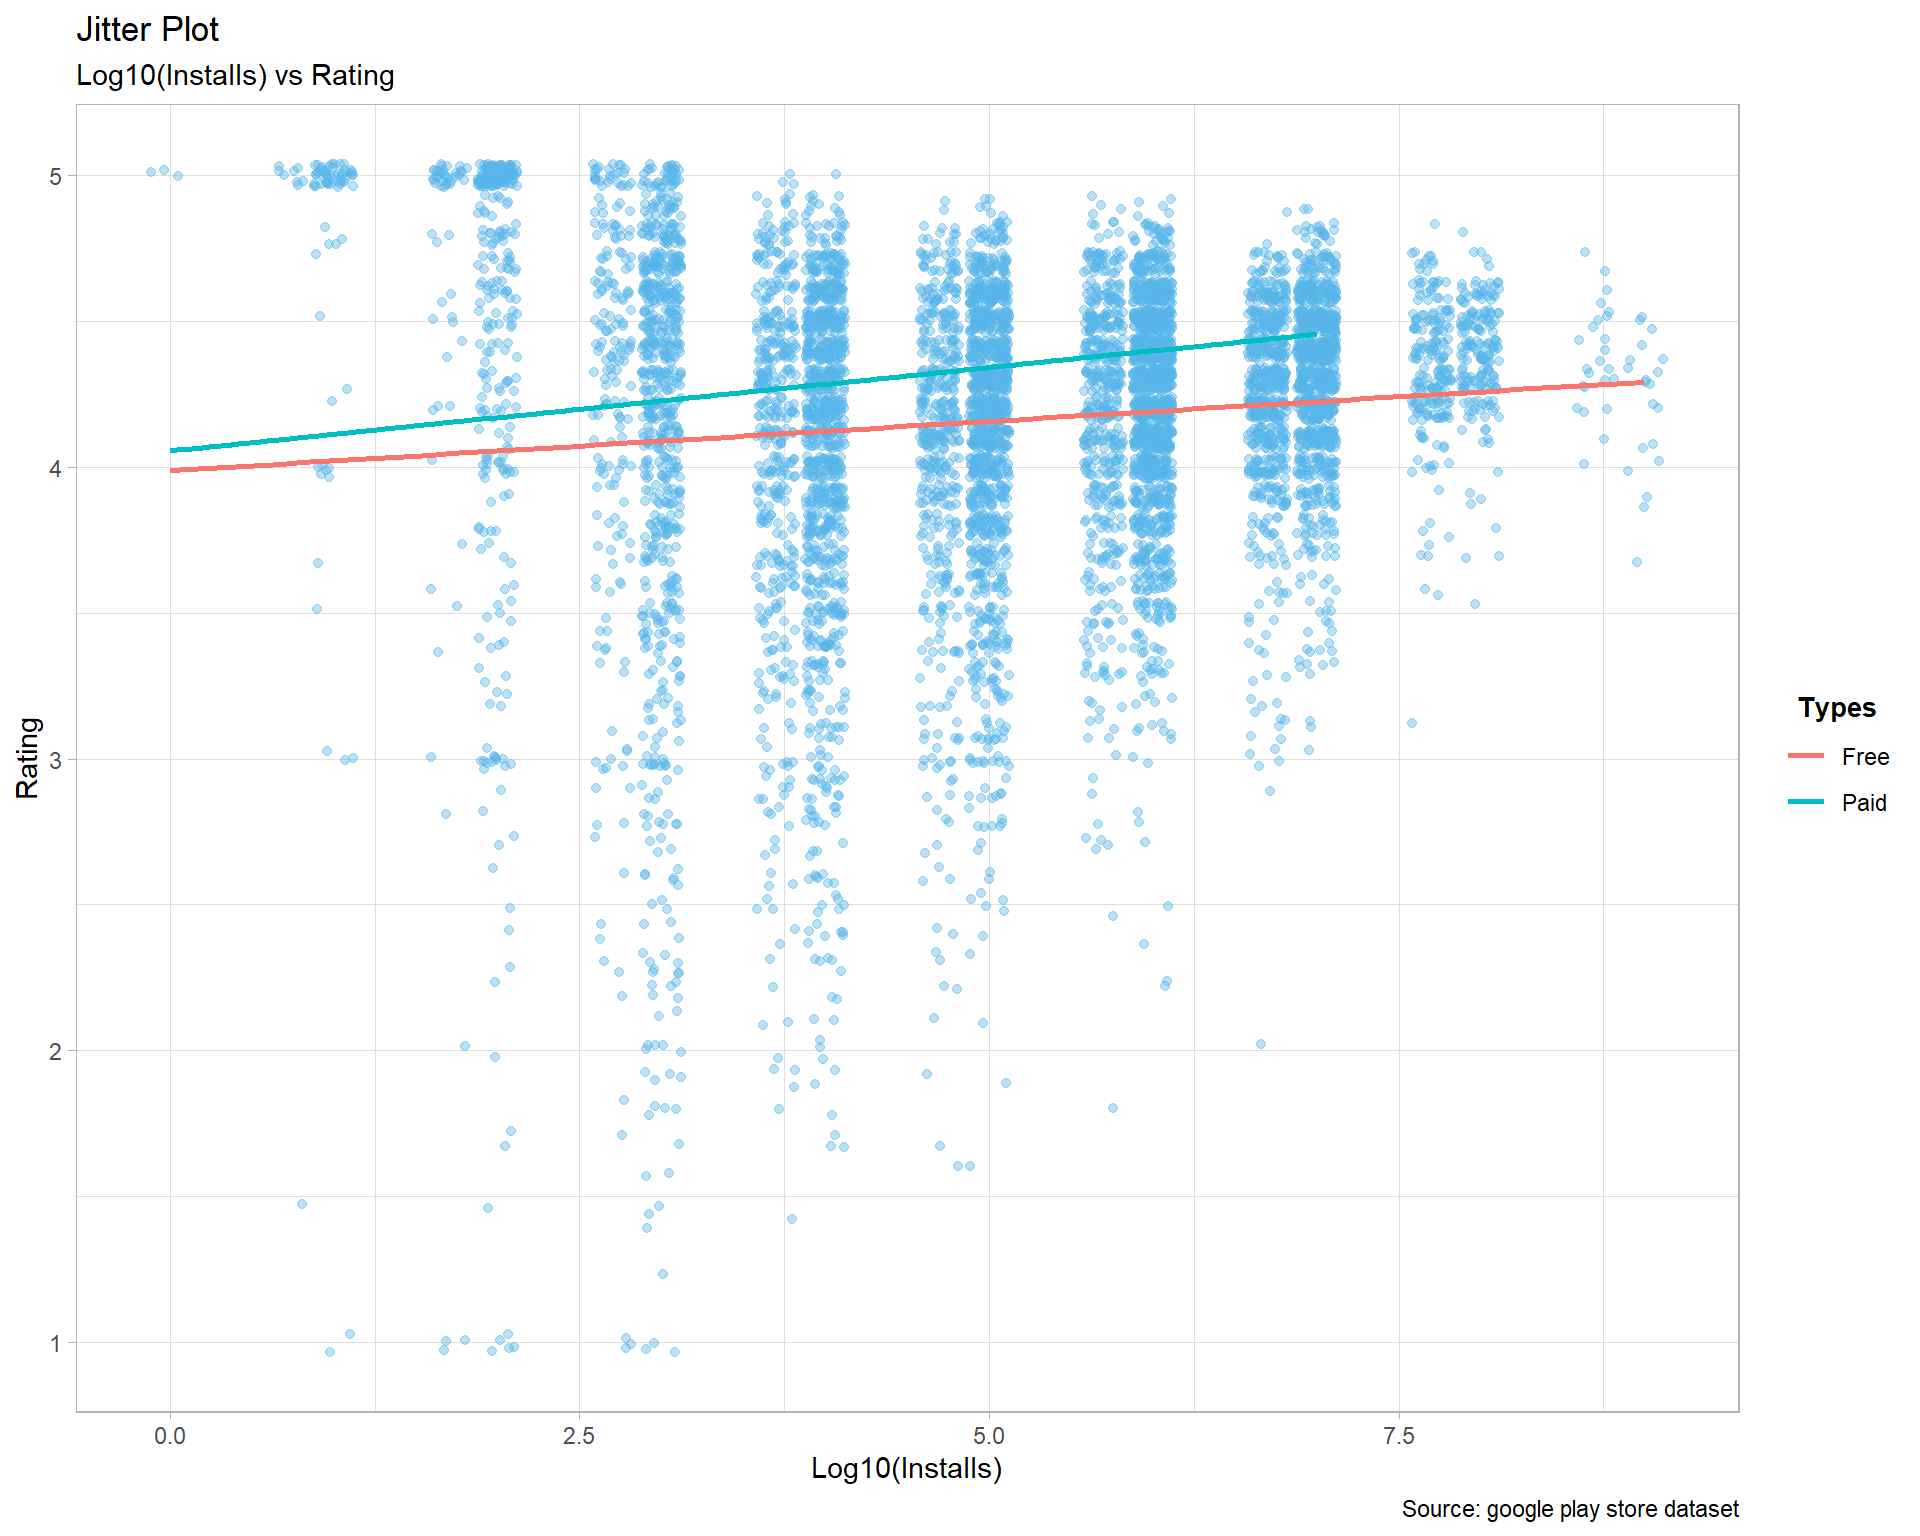
\includegraphics{Group3_final_report_files/figure-latex/descriptive_modeling_2-1.pdf}

\textbf{Observations/Findings}: We observed that the rating of paid
applications is much higher than the free apps. Which might be indicate
its better quality. On the other hand, Free apps have a higher number of
installs, thus covering a wide range of audience.

\hypertarget{cross-validation-of-models}{%
\subsection{Cross Validation of
models}\label{cross-validation-of-models}}

This technique helps us identify the best fit model for our dataset
i.e.~the model with least root mean square error

\begin{verbatim}
## [1] 0.5130422
\end{verbatim}

\begin{verbatim}
## [1] 0.5031791
\end{verbatim}

\begin{itemize}
\tightlist
\item
  We sliced the dataset into training and test dataset. Training data
  det contain 6951 observations (75\% of total) and test data set
  contains 2198 observations (25\% of total).
\item
  We trained both lm model and rpart model with the training dataset.
\item
  After training the model we predicted the rating values for test
  dataset. In order to find which model did a better job of predicting
  the value of rating, we calculated the root mean square error (RMSE)
  for the predictions made by both models. RMSE values for lm and rpart
  are 0.5476666 and 0.5399403 respectively. We can see that RMSE value
  for rpart is less than RMSE value for lm, implying that rpart can make
  a better prediction than lm.
\item
  Along with performing a comparison between lm and rpart, we
  experimented with different explanatory variables. We got the least
  RMSE by using installs, types, categories and reviews as explanatory
  variables.
\end{itemize}

\hypertarget{making-predictions}{%
\subsection{Making Predictions}\label{making-predictions}}

We can predict rating of a dummy app by entering different parameters
like installs, types, category and reviews

\begin{verbatim}
##        1 
## 4.294068
\end{verbatim}

\begin{verbatim}
##        1 
## 4.132784
\end{verbatim}

\begin{itemize}
\tightlist
\item
  \textbf{1st dummy application}: First dummy application of type Free
  with 1 billion installs and 100000 reviews, belonging to TOOLS
  category has a predicted rating of 4.2884. This seems like a
  reasonable prediction A Free app with 1 billion installs and 100,000
  reviews must be a popular app and is expected to have high rating. But
  the fact that it belongs to ``Tools'' category, which has the third
  least average rating, its rating is not exceptionally high. Its rating
  much better than average (4.17) but is not among the highest ratings.
\item
  \textbf{2nd dummy application}: Second dummy application is of type
  Free, with 1000 installs and 100 reviews, belonging to EVENTS
  category, has a predicted rating of 4.0436. This seems like a
  reasonable prediction. A free app is expected to have higher installs,
  but as this app does not have high number of installs, indicating that
  the app is not the best in its segment or it has limited relevance or
  utility, thus we can expect low rating. But, as it belongs to EVENTS
  category, which has the highest average rating among all categories,
  its rating is not among the worst. It has a below average rating but
  is still not among the wort rated apps.
\end{itemize}

\hypertarget{conclusion-1}{%
\section{Conclusion}\label{conclusion-1}}

\hypertarget{references}{%
\section{References}\label{references}}

{[}1{]}
\href{https://www.kaggle.com/lava18/google-play-store-apps}{Dataset};\\
{[}2{]}
\href{https://bookdown.org/yihui/rmarkdown/html-document.html\#tabbed-sections}{R
markdown} ;\\
{[}3{]}
\href{https://stackoverflow.com/questions/3993301/how-to-format-number-values-for-ggplot2-legend/15007117}{Stackoverflow}
;\\
{[}4{]}
\href{https://ggobi.github.io/ggally/rd.html\#ggpairs}{GGally};\\
{[}5{]}
\href{https://drsimonj.svbtle.com/creating-corporate-colour-palettes-for-ggplot2}{Custom
color pallete};\\
{[}6{]} {[}7{]}
\href{https://hbr.org/2014/04/the-right-colors-make-data-easier-to-read}{Colors};\\
{[}8{]} \href{https://www.tidyverse.org/}{TidyVerse};\\
{[}9{]} \href{https://ggplot2.tidyverse.org/reference/}{ggplot2};\\
{[}10{]}
\href{https://www.kaggle.com/danilodiogo/google-play-store-eda-plotting-with-highcharts/code\#eda}{Google
playstore Kernel by Danilodiogo};\\
{[}11{]}
\href{https://gs.statcounter.com/os-market-share/mobile/worldwide}{market
share} ;\\
{[}12{]} \href{https://globalgamejam.org/}{Global game jam} ;\\
{[}13{]}
\href{https://www.statista.com/statistics/266210/number-of-available-applications-in-the-google-play-store/}{Play
Store Statistics} ;

\end{document}
